\documentclass[a4paper,12pt]{book}
\usepackage{kotex}

\usepackage{amsmath}
\usepackage{amsfonts}
\usepackage{amssymb}
\usepackage[toc,page]{appendix}
\usepackage{array}
\usepackage{atbegshi}
\usepackage{bookmark}
\usepackage{caption}
\usepackage{color}
\usepackage{cleveref}
\usepackage[
    type={CC},
    modifier={by},
    version={4.0},
]{doclicense}
\usepackage{enumitem}
\usepackage{etoolbox}
\usepackage{fancyhdr}
\usepackage{fancyvrb}
\usepackage{float}
\usepackage{graphicx}
\usepackage{hyphenat}
\usepackage{listings}
\usepackage{longtable}
\usepackage[framemethod=tikz]{mdframed}
\usepackage{microtype}
\usepackage{scrlayer}
% \usepackage{setspace}
\usepackage{tikz}

\usepackage{hyperref}

\usetikzlibrary{patterns,positioning}

% THEOREM

\newtheorem{exercise}{Exercise}

% MACROS

\newcommand{\cnote}[1]{
    \marginpar{
        \linespread{1}
        \begin{tikzpicture}[pin]
            \foreach \X in {0,...,22} {
                \foreach \Y in {-2,...,2}
                    \filldraw[color=red!45] (\X*2pt+\Y*\Y,-\Y*2pt-4pt) circle ({(5-0.2*\X)*0.1pt});
            }
            \draw (48pt,-4pt) node[right] {\small NOTE};
        \end{tikzpicture}
        \small{#1}
    }
}
\newcommand{\Mod}[1]{\ (\mathrm{mod}\ #1)}
\newcommand{\V}[1]{\Verb|#1|}
\newcommand{\Ve}[1]{\Verb+#1+}
\newcommand{\exercise}[1]{
    \begin{exercise} 
        #1 
    \end{exercise}
}
%\newcommand*{\fullref}[1]{\namecref{#1} `\nameref*{#1}'}
\newcommand*{\fullref}[1]{\autoref{#1} (\nameref*{#1})}

\newcommand{\ccomment}[1]{}

% LSTLISTING

\definecolor{light-gray}{gray}{0.95}
\definecolor{gray}{gray}{0.4}
\lstset{
    columns=fullflexible,
    inputencoding=utf8,
    escapeinside={(*@}{@*)},
    basicstyle=\linespread{1}\small\ttfamily
}
\surroundwithmdframed[
  hidealllines=true,
  backgroundcolor=light-gray,
  innerleftmargin=15pt,
  innertopmargin=0pt,
  innerbottommargin=0pt]{lstlisting}

% STYLES

\AtBeginEnvironment{quote}{\par\singlespacing}

\setlist[enumerate]{noitemsep}
\setlist[itemize]{noitemsep}
\AtBeginEnvironment{enumerate}{\linespread{1}}

%================================%
% DOCUMENT                       %
%================================%

\title{Introduction to C Programming Language}
\author{서영원}
\date{April 2024}
\begin{document}

\linespread{1.5}

\maketitle

\tableofcontents

\vfill
\doclicenseThis


\pagebreak

\microtypesetup{activate=false}

%================================%

\chapter{들어가기에 앞서}

%================================%

\section{작가의 말}

본 도서는 독자가 고1 수준 수학의 개념을 모두 알고 있다는 전제 하에 서술되었다.
혹여나 모른다고해서 걱정하지 말라, 모두 쉽게 풀어 설명되어있다.

글을 읽다보면 이곳 저곳에 개념의 역사 등 자잘한 것들을 서술하는 방주(旁註)가 작성되어있다.
딱히 읽어야만 하는 것은 아니지만, 교양과목을 듣는다는 마음으로 찬찬히 읽어보도록 하자.

%================================%

\section{사전 준비}

\textit{제작 플랫폼 간단 소개 (회원가입 등)}

%================================%

\chapter{시작하기}

%================================%

\section{C언어의 탄생}

운영체제와 브라우저, 온갖 응용프로그램들까지 현대에 이르러 더이상
C언어의 손길을 거치지 않은 프로그램은 없다.
컴퓨터는 인간이 이해할 수 있는 언어는 이해하지 못한다고들 하는데,
그렇다면 C언어는 어떻게 컴퓨터 시스템에서 실행될 수 있을까?
인간이 지금껏 사용해온 언어, 자연어는 왜 컴퓨터 시스템에서 사용되지 않는
것일까?

%================================%

\subsection{자연어의 모호성}

\begin{quote}
`마트가서 우유사고 만약에 아보카도 있으면 6개 사와'
\end{quote}

오늘 독자가 아내로부터 하달받은 명령이다.
우리는 이를 해석함에 있어서 다음과 같이 2가지 해석을 마련할 수 있다.

\begin{center}

    \centering

    아보카도 명령 코드

    \begin{minipage}{0.45\textwidth}
        \begin{lstlisting}[escapeinside=``]
`마트로 이동한다.`
`우유 1개 구매한다.`
`만약 아보카도가 진열되어있다면:`
    `아보카도 6개 구매한다.`
        \end{lstlisting}
    \end{minipage}
    \hfill
    \begin{minipage}{0.45\textwidth}
        \begin{lstlisting}[escapeinside=``]
`마트로 이동한다.`
`만약 아보카도가 진열되어있다면:`
    `우유 6개 구매한다.`
`아니라면:`
    `우유 1개 구매한다.`
        \end{lstlisting}
    \end{minipage}

\end{center}

만에 하나 둘 중에 잘못된 선택지를 골랐다면 (우유 6팩을 구매한다는 둥)
감히 끔찍한 일이 닥치고 말 것이다.

마찬가지로, 컴퓨터를 프로그램함\footnote{프로그램을 컴퓨터에 내장하는 \\
행위}에 있어서 이러한 모호성이 존재할 경우 이가 실행될 때에 컴퓨터는 둘
중 어떠한 행위를 해야할 지 선택해야만 한다. 이는 사용자가 의도하지 않은
동작을 초래할 수 있는 매우 위험한 상태다. 따라서, 그 자체로 모호성을
내재한 자연어는 컴퓨터를 프로그램하기 위한 언어로 적절하지 못하다.

%================================%

\subsection{명령집합과 기계어}

\begin{table}[!h]
    \centering

    \caption{아보카도 명령 집합}
    \label{Tab:avocado-isa}

    \begin{tabular}{ || m{2em} | m{3.8em} | m{22em} || }
        \hline
        이름 & 매개변수 & 동작 \\
        \hline\hline
        buy & 물품 t, 자연수 n & t를 n개 만큼 구매한다. 아니라면 0으로 정의한다 \\
        \hline
        find & 물품 t & 물품 t가 존재한다면 r을 1로 정의한다. 아니라면 r을 0으로 정의한다. \\
        \hline
        move & 위치 p & r이 0이라면 위치 p로 이동한다. 아니라면 아무 동작도 하지 않는다. \\
        \hline
    \end{tabular}
    \newline
    \textit{\color{gray} \small r은 미지수 내지 변수라고 정의하자.
    아직 너무 엄밀해질 필요는 없다.}
\end{table}

대신, 컴퓨터는 인위적으로 정의된 명령 집합에 따라 작동한다.
우리도 컴퓨터처럼 아내에게 더욱 엄밀하고 덜 모호하게 명령을 내려달라고 요구하기 위해,
아보카도와 우유를 향한 임무 달성을 위해 \autoref{Tab:avocado-isa} 과 같이 명령
집합을 정의해보자.

이러한 명령집합을 사용하면 아래와 같이 \textbf{엄밀하게} 우리의 행위를
정의해볼 수 있다. (명령은 위에서부터 순차적으로 실행한다.)

\begin{center}

    \centering

    아보카도 명령 코드 (최종)

    \begin{minipage}{0.45\textwidth}
        \begin{lstlisting}[escapeinside=``]
buy(`우유`, 1)
find(`아보카도`)
move(`출구`)
buy(`아보카도`, 6)
        \end{lstlisting}
    \end{minipage}
    \hfill
    \begin{minipage}{0.45\textwidth}
        \begin{lstlisting}[escapeinside=``]
buy(`우유`, 1)
find(`아보카도`)
move(`출구`)
buy(`우유`, 5)
        \end{lstlisting}
    \end{minipage}

\end{center}

이렇게만 적어도 사람이 프로그램을 수행함에 있어서 어려움은 없다.
그러나, 전류 흐름의 여부로 신호를 처리하는 컴퓨터에게 있어서,
한글과 알파벳을 이해하도록 하는 것은 매우 복잡할 것이다.
% (컴퓨터가 어떻게 글자를 처리하는 지에 대해선 뒤 \fullref{sec:code-page}와 \fullref{sec:fonts}를 참조하라)

따라서, 우리는 다음과 같이 각각의 명령과 단어들에 번호를 부여할 것이다.

\begin{table}[!h]
    \centering

    \caption{아보카도 명령 집합 (최종)}
    \label{Tab:avocado-isa-int}

    \begin{tabular}{ || c | c | c | c || }
        \hline
        이름 & 번호 & 이름     & 번호 \\
        \hline\hline
        buy  & 0    & 아보카도 & 0    \\
        \hline
        find & 1    & 우유     & 1    \\
        \hline
        move & 2    & 출구     & 2    \\
        \hline
    \end{tabular}
\end{table}

부여된 번호를 통해 다시 구현하면 다음과 같다.

\begin{center}

    \centering

    아보카도 명령 코드 (진짜최종)

    \begin{minipage}{0.45\textwidth}
        \begin{lstlisting}
0(1, 1)
1(0)
2(2)
0(0, 6)
        \end{lstlisting}
    \end{minipage}
    \hfill
    \begin{minipage}{0.45\textwidth}
        \begin{lstlisting}
0(1, 1)
1(0)
2(2)
0(1, 5)
        \end{lstlisting}
    \end{minipage}

\end{center}

또한 다음의 규칙에 따라 명령을 기계가 이해하기 쉽도록 바꾸어보자.

\begin{itemize}
    \item 명령과 상품에는 각각 두자리를 할당하자
    \item 상품의 갯수에는 네자리를 할당하자
\end{itemize}

결과는 다음과 같다:

\begin{center}

    \centering
    
    아보카도 명령 코드 (진짜최종2)

    \begin{minipage}{0.45\textwidth}
        \begin{lstlisting}
00 01 0001
01 00
10 10
00 00 0110
        \end{lstlisting}
    \end{minipage}
    \hfill
    \begin{minipage}{0.45\textwidth}
        \begin{lstlisting}
00 01 0001
01 00
10 10
00 01 0101
        \end{lstlisting}
    \end{minipage}

\end{center}

축하한다! 독자는 방금 마트에 가서 우유 (혹은 아보카도)를 구매하기위한
명령 체계\footnote{Instruction Set Architecture를 줄여 ISA라고도 부른다.}를 완성했다!
이제 독자는 독자의 아내에게 \textbf{모호하지 않은} 명령을 내려달라고 요구할 수 있을 것이다!

%================================%

\subsection{기계어와 C언어}

\cnote{
    어셈블리어는 Maurice Wilkes, David Wheeler와 Stanley Gill의 저서
    \textit{The Preparation of Programs for an Electronic Digital Computer}
    에서 최초로 제시되었다.
    본 도서에는 이 외에 최초로 \textit{재사용 가능한} 코드, \textit{API},
    디버깅을 위해 \textit{메모리 덤프}를 사용하는 방법이 서술되었다.
}

...그래서 이 기계어가 C언어랑 무슨 상관일까?
그것은 C언어의 태생에 있다.
자세히 알아보기 위해 1951년으로 돌아가보자.

%================================%

\subsubsection{복잡해지는 ISA와 어셈블리어}

| 컴퓨터를 프로그램하기 위해 0과 1만 두드리고 있는 것은
매우 지루한 일일 뿐더러, 코드에 오류가 존재하거나 오타를 치고 말았을때
수정하기 매우 번거롭다.

개발자들은 이러한 문제를 해결하기 위해
\textit{어셈블리어}\footnote{ASseMbly language를 줄여 ASM이라고 부른다.}를 도입했다. 


이는 독자가 설계한 `아보카도 명령 코드 (최종)'과 비슷한 것으로,
기계어에 일대일 대응되도록 알파벳으로 이루어진 이름을 부여한 것이다.

다음의 규칙과 함께 아래의 명령을 해석해보자:

\begin{table}[!h]
    \centering

    \caption{계산기 ISA}
    \label{Tab:simple-calculator-isa}

    \begin{tabular}{ || m{2em} | m{5em} | m{22em} || }
        \hline
        이름 & 매개변수 & 동작 \\
        \hline\hline
        add  & 값 t & 변수 a에 t만큼 더한 값을 a로 정의한다 \\
        \hline
        mul  & 값 t & 변수 a와 t를 곱한 값을 a로 정의한다 \\
        \hline
        div  & 값 t & 변수 a를 t로 나눈 값을 a로 정의한다 \\
        \hline
        mov  & 변수 a, 값 v & a에 v를 대입한다 \\
        \hline
    \end{tabular}
\end{table}

\begin{center}

    \centering
    
    \autoref{Tab:simple-calculator-isa}를 이용한 코드

\begin{lstlisting}
mov b, a
add 1
mul b
div 2
mov b, a
\end{lstlisting}
\end{center}

위의 코드는 정의된 ISA에 따라 아래와 같은 수식으로 해석할 수 있다:

\begin{equation}
b = \frac{a(a + 1)}{2}
\end{equation}

하지만, 세상에 이렇게 간단한 코드만 존재했다면 세상은 지금까지조차 ASM을
쓰고 있을지도 모르겠다.
그럼 그렇지, 요즘 많이 사용되는 x86-64 구조는 명령어 약 3,600개 가량을
가지고 있다.
이 것들을 아무런 도움도 없이 활용하여 성능 좋고 보기도 좋은 프로그램을
만드는 것은 매우 어려운 일이다.

%================================%

\subsubsection{고수준 언어의 등장}

| 개발자들은 \textbf{사람이 이해하기 쉬운} 프로그래밍 언어를 원했다.
결국 1953년, IBM의 John Backus는 세계 최초의 고수준 프로그래밍 언어,
\textit{Speedcoding}을 개발했다.

\begin{figure}[!h]
    \centering
    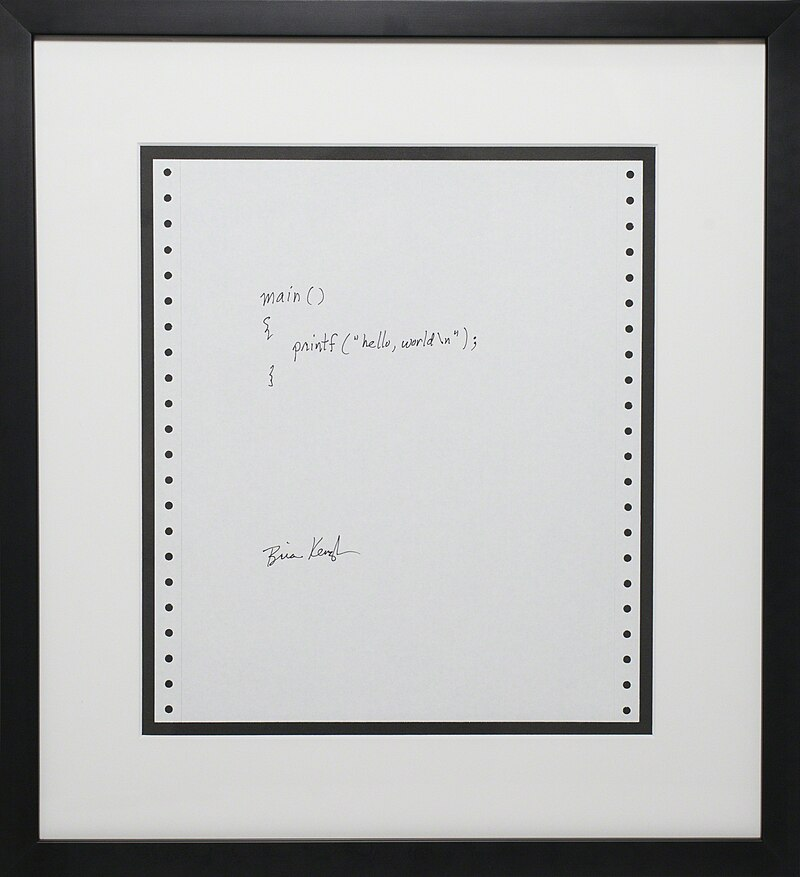
\includegraphics[width=\linewidth]{images/hello-world.jpg}
    \caption{1978년, C언어를 공동개발한 Brian Kernighan의 Hello, World}
\end{figure}

이후 \textit{Fortran}(1957), \textit{ALGOL}(1960), \textit{CPL}(1963)과
\textit{B}(1969)를 거치고, 드디어 1972년 벨 연구소, Dennis Ritchie는
\textit{C}를 개발한다.

\pagebreak

%================================%

\section{Hello, World!}

C언어는 기본적으로 ASM과 같은 저급언어을 추상화하기 위해 태어난 여러 언어들의 문제점들을 해결하기 위해 만들어졌다.
따라서, C언어의 문법을 이해하기 위해, 먼저 초보자를 위해 설계된 BASIC으로 작성된 예제를 살펴보자.

(본 단원은 반복문, 함수의 개념을 언어의 발전과정을 통해 이해하기 쉽게 하기 위한 단원이다.
이미 반복문, 조건문, 함수의 개념을 알고있다면, 곧바로 \fullref{sec:hello-c}로 넘어가도 좋다!)

%================================%

\subsection{Hello, BASIC!}

\begin{lstlisting}
10 PRINT "Hello, BASIC!"
20 END
\end{lstlisting}

위는 BASIC을 통해 화면에 `Hello, BASIC!'라는 문장을 출력하는 예제다.

영어를 할줄 안다면 대충 이해했을텐데, 
첫 줄의 \V{PRINT ``Hello, BASIC!"}는 `Hello, BASIC!'라는 문장을 출력하도록 하는 명령,
두번째 줄의 `END'는 프로그램이 종료되었음을 알리는 명령이다.

\exercise{위 코드를 직접 실행해보자!}
\exercise{\V{Hello, BASIC!}대신에 다른 문장을 넣어보고, 어떻게 되는지 확인해보자!}

%================================%

\subsection{더 깊은 곳으로}

더 복잡한 예시를 살펴보자.

\begin{lstlisting}
10 N=100
20 FOR I=1 TO N
30 PRINT "Hello, BASIC!"
40 NEXT I
\end{lstlisting}

위의 예시는 다음의 과정에 따라 \V{Hello, BASIC!}라는 문장을 100번 출력하는 예제다:

첫 줄의 명령:

\begin{lstlisting}
10 N=100
\end{lstlisting}

는 변수 \V{N}의 값을 100으로 정의한다.

\begin{lstlisting}
20 FOR I=1 TO n
...
40 NEXT I
\end{lstlisting}

에서, \V{FOR I=1 TO N}은 변수 I이 1에서 N까지 이산적으로 증가
($\textstyle \sum\limits_{I=1}^N$)하는 동안,
`\V{...}'에 있는 명령들을 실행하도록 한다.
이렇게, 어떤 명령들을 쉽게 반복할 수 있게 해주는 구문을 `반복문(loop)'이라고 한다.

다음 줄의 구문:

\begin{lstlisting}
30 PRINT "Hello, BASIC!"
\end{lstlisting}

은 \V{Hello, BASIC!}이라는 문장을 출력한다.

\exercise{N과 I의 값을 변경하고, 출력이 어떻게 변화하는지 살펴보자!}

%================================%

\subsection{입력 받기}

BASIC에서 출력 뿐만 아니라, 입력을 받아볼 수도 있지 않을까?
다음의 예시를 살펴보자:

\begin{lstlisting}
10 INPUT "How many stars? "; C
20 S$ = ""
30 FOR I=1 TO C
40 S$ = S$ + "*"
50 NEXT I
60 PRINT S$
70 INPUT "Do you want more? "; A$
80 IF LEN(A$) = 0 THEN GOTO 70
90 IF A$ = "y" OR A$ = "Y" THEN GOTO 10
100 PRINT "Goodbye"
110 END
\end{lstlisting}

\begin{lstlisting}
10 INPUT "How many stars? "; C
\end{lstlisting}

는 `\V{How many stars? }'를 출력하고, 입력값을 변수 C에 저장한다.

\begin{lstlisting}
20 S$ = ""
\end{lstlisting}

는 변수 \V{S\$}의 값을 빈 문자열 \V{``''}로 정의한다.

\begin{lstlisting}
30 FOR I=1 TO C
40 S$ = S$ + "*"
50 NEXT I
\end{lstlisting}

는 변수 \V{I}의 값을 1에서 \V{C}까지 변화시키며,
변수 \V{S\$}의 뒤에 \V{*}를 한글자씩 덧붙인다.

\begin{lstlisting}
60 PRINT S$
\end{lstlisting}

는 현재 \V{S\$}의 값을 출력한다.

\begin{lstlisting}
70 INPUT "Do you want more? "; A$
\end{lstlisting}

는 `\V{Do you want more? }'을 출력하고,
입력값을 변수 \V{A\$}에 저장한다.

\begin{lstlisting}
80 IF LEN(A$) = 0 THEN GOTO 70
\end{lstlisting}

위 구문은 아래와 같이 해석할 수 있다:

\begin{itemize}
    \item `\V{IF ... THEN ...}'는 \V{IF}뒤의 조건이 만족되었을때,
    \V{THEN}뒤의 명령을 수행한다.
    이렇게 조건에 따라 명령의 수행 여부를 결정하는 구문을 `조건문'이라고 한다.
    \item \V{LEN(A\$)}는 변수 `\V{A\$}'의 길이(글자의 개수)를 의미한다.
    \item `\V{GOTO 70}'은 70번째 줄(명령 앞에 붙은 번호)로 이동하라는 의미이다.
\end{itemize}

따라서, 입력(\V{A\$})의 글자수가 0이라면, 70번째 줄로 이동하라는 의미이다.

\begin{lstlisting}
90 IF A$ = "y" OR A$ = "Y" THEN GOTO 10
\end{lstlisting}

는 입력(\V{A\$})가 \V{y} 또는(\V{OR}) \V{Y}라면, 10번째 줄로 이동하라는 의미이다.

\begin{lstlisting}
100 PRINT "Goodbye"
110 END
\end{lstlisting}

는 \V{Goodbye}를 출력하고, 프로그램을 종료하라는 의미이다.

결국, 위 프로그램은 입력받은 숫자만큼 `*'을 출력하는 프로그램이다.
프로그래밍에 익숙하지 않거나, `goto'를 사용해본적 없다면, 위 코드부터 슬슬 어지러움을 느낄 수 있다.
물론, 아직까지 어지럼증을 느끼지 않을 순 있으나, `*'와 `-' 중 선택한 문자를 출력하도록 하는 프로그램이라던지,
여러 기능들을 추가하다보면 점점 내가 뭘 하고있는지 알수 없게되는 시점이 온다.

이를 해결하기 위해 개발자들은 언어를 `구조화'시키기 시작했다.

%================================%

\subsection{Label과 Goto}

개발자는 먼저 줄번호(명령의 앞에 붙어 명령의 번호와 순서를 지정하는 번호)를 없애고, 대신 `레이블(label)'을 도입했다.
예를 들면 다음과 같다:

\begin{center}

    \centering
    
    줄번호를 이용한 BASIC(좌)과 label을 이용한 BASIC(우)

    \begin{minipage}{0.45\textwidth}
        \begin{lstlisting}
10 PRINT "Hello!"
20 GOTO 10
        \end{lstlisting}
    \end{minipage}
    \hfill
    \begin{minipage}{0.45\textwidth}
        \begin{lstlisting}
Print:
PRINT "Hello!"
GOTO Print
        \end{lstlisting}
    \end{minipage}

\end{center}

\cnote{
    Syntax Sugar:
    없으면 프로그램을 구현하지 못하는게 아닌데도, 사람이 표현하기 쉽도록 설계된 문법.
}

훨씬 가독성이 좋아진 모습이나,
`GOTO'가 코드에 보이는 것 조차 싫었던 개발자들은 `GOTO'없이 코드를 작성하기 위해 여러 문법 설탕들과 `서브루틴(subroutine)'의 개념을 추가했다.

%================================%

\subsection{DO WHILE ... LOOP}

2세대 BASIC언어들에는 참 많은 문법 설탕들이 있지만,
그중에서도 `DO WHILE ... LOOP'를 소개하고자 한다.

\begin{center}
    \centering

    `\V{GOTO}'(상)와 `\V{DO WHILE ... LOOP}'(하)

\begin{lstlisting}
Print:
PRINT "Hello, BASIC!"
INPUT "Want one more line? "; S$
IF S$ = "y" OR S$ = "Y" THEN GOTO Print
\end{lstlisting}
\begin{lstlisting}
PRINT "Hello, BASIC!"
INPUT "Want one more line? "; S$
DO WHILE S$ = "y" OR S$ = "Y"
    PRINT "Hello, BASIC!"
    INPUT "Want one more line? "; S$
LOOP
\end{lstlisting}

\end{center}

label을 없애고 WHILE을 통해 직관적으로 반복문의 구조와 조건을 밝히며 가독성을 높이고 있다.
그러나, 같은 명령이 두번씩 반복되는 것은 그다지 좋지 않은 코드다.
%(`그다지 좋지 못한 코드'가 무엇인지 궁금한 독자는 \fullref{sec:clean-code}를 참조하라.)
이런 상황을 위해 `DO ... LOOP WHILE'문이 준비되어있다.



\begin{center}
    \centering

    `\V{DO WHILE ... LOOP}'(상)와 `\V{DO ... LOOP WHILE}'(하)

\begin{lstlisting}
PRINT "Hello, BASIC!"
INPUT "Want one more line? "; S$
DO WHILE S$ = "y" OR S$ = "Y"
    PRINT "Hello, BASIC!"
    INPUT "Want one more line? "; S$
LOOP
\end{lstlisting}
\begin{lstlisting}
S$ = ""
DO
    PRINT "Hello, BASIC!"
    INPUT "Want one more line? "; S$
LOOP WHILE S$ = "y" OR S$ = "Y"
\end{lstlisting}

\end{center}

반복문 내의 코드를 실행하기 이전에 조건을 검사해, 두번씩 작성되던 코드를 한번만 작성할 수 있게 했다.

이와 같이 BASIC과 많은 언어들은 문법 설탕을 첨가하며 발전해왔고, C언어 또한 이러한 구조들을 채택하고 있다.
이제 서브루틴에 대해 알아보자.

%================================%

\subsection{서브루틴}

특정한 갯수 만큼 별표(`*')를 출력하는 등 자주 반복되는 명령들을 하나로 묶어서 사용할 순 없을까?
묶어서 사용할 수만 있으면, 같은 명령어들이 반복해서 쓰이는 상황들도 효과적으로 줄일 수 있을 것이다.

이러한 고민 속에 탄생한 것이 서브루틴으로,
단순히 말하자면, 특정한 일을 처리하기 위해 일련의 명령어들을 묶어둔 것이다.

쉬운 이해를 위해 BASIC코드를 보며 이해해보자:

\begin{lstlisting}
10 GOSUB 100
20 PRINT "Bye, SUBROUTINE!"
30 END
100 PRINT "Hello, SUBROUTINE!"
110 RETURN
\end{lstlisting}

위 코드에서 `GOSUB 100'은 `GOTO'와 같이 줄번호 100으로 점프하고,
`PRINT ``Hello, SUBROUTINE!"'과 `RETURN'을 순차적으로 실행시킨다.
유일한 차이점은, `RETURN'이 실행되면 줄번호 10의 자리로 돌아와
'PRINT ``Bye, SUBROUTINE!"을 실행한다는 것이다.

이와 같이 서브루틴은 특정한 주소 공간에 명령어를 모아서 작성할 수 있게 하고,
이를 통해 코드의 유지보수를 쉽게 만들어준다.

그러나, 기술이 발전하고 BASIC에서 줄번호를 없애는 과정속에서 `GOSUB' 또한 개량되어야 했다.
이를 해결하기 위해 개발자들은 `함수(function)'이라는 개념을 도입했다.

%================================%

\subsection{함수}

독자가 한국인이라면, 함수는 중학교에서 알게된 수학 용어일 것이다.
프로그래밍에서의 `함수'또한 비슷한 의미로,
입력을 받아 (정의역에 대해) 일을 처리하기 위해 (출력을 가지기 위해; 치역을 가지기 위해)
묶어놓은 일련의 명령어 묶음이다. (물론, 입력을 받지 않아도 좋다. 이에 대해선 후술한다.)

BASIC에서는 함수를 다음과 같이 작성한다:

\begin{lstlisting}[escapeinside=``]
SUB `함수명`(`매개변수1`, `매개변수2`, ...)
    `명령어...`
END SUB
\end{lstlisting}

위에서 `GOSUB'와 함께 서술된 코드를 함수 문법을 통해 다시 작성해보자:

\begin{lstlisting}
CALL PrintHello()
PRINT "Bye, SUBROUTINE!"
END

SUB PrintHello()
    PRINT "Hello, SUBROUTINE!"
END SUB
\end{lstlisting}

위와 같이, 그저 반복되는 명령어들을 하나로 함축하기 위함이라면 매개변수,
즉 입력을 받지 않아도 좋다.

%================================%

\subsection{Hello, C!}
\label{sec:hello-c}

C언어는 상술된 개념들을 대부분 문법적인 개량만 가지고 차용하고 있다.
이제 C언어를 통해 `Hello, World!'를 출력해보자!


\begin{lstlisting}
#include <stdio.h>

int main()
{
    printf("Hello, World!\n");
    return 0;
}
\end{lstlisting}

위 C언어 코드는 아래의 BASIC 코드와 동일하다:

\begin{lstlisting}
CALL main()

SUB main()
    PRINT "Hello, World!"
END SUB
\end{lstlisting}

C언어에서는 함수를 정의하는데에 있어서,
서브루틴이라는 개념보다 본격적으로 수학에서의 함수를 닮았다.

수학에서 함수를 $f(x) = ...$와 같이 서술했던 것과 비슷하게,
C언어에서도 함수를 \V{f(x) \{ ... \}}라고 작성한다.
(매개변수는 여럿일 수 있다; \V{f(a, b, c)}라고 작성한다)

\V{main}앞의 \V{int}는 이러한 맥락에서 추가된 것이다.
암시적으로 함수의 공역을 알 수 없기 때문에,
명시적으로 \V{main}의 공역이 \V{int}(\textit{integer}의 축약어; 이에 대해선 후술한다)
임을 표기한 것이다.

\V{return 0;}는 \V{main}의 반환값을 0이라고 선언한 것으로,
\V{main}의 반환값에 따라 프로그램을 실행한 OS는
프로그램이 정상적으로 종료되었는지 판단하게 된다.

그럼, 정의역은 어디있을까?
C언어에서는 함수의 정의역이 존재하지 않아도 좋다.
\cnote{
    사실, \V{main(void)}와 \V{main()}은 다르다.
    \V{main()}은 가변길이의 매개변수를 수용하는데,
    궁금한 독자는 ANSI C표준에 대해 찾아보라.
}
\cnote{
    C언어는 \textit{상태기계}이기 때문에,
    매개변수가 곧 정의역인 것은 아니다.
    궁금한 독자는 \textit{상태기계}에 대해 찾아보라.
}
이러한 경우 \V{main(void)}라고 작성하기도 하는데,
수학적으로 엄밀히 바라보고싶다면,
$main : \{ void \} \rightarrow \mathbb{Z}$와 같이 생각해도 좋다.
(이때 \V{void}는 어떤 문법적 의미를 가지지 않는, 길이가 0인 문자열이다)
따라서, \V{main()}은 매개변수를 가지지 않는 `main'이라는 이름의 함수를 선언한 것이고,
그 밑의 \V{\{ ... \}}는 이 함수가 어떤 일을 하는지 서술한다.

따라서, 위의 C언어 코드의 \V{main()}은 호출되었을때,
`\V{Hello, World!\textbackslash{}n}'
(\textbackslash{}n는 개행을 표현하기 위한 특수문자다.
자세한 내용은 \fullref{sec:escapes}를 참조하라.)
를 출력하는 함수라고 말할 수 있다.

`\V{\#include <stdio.h>}'는
이 프로그램이 표준(std; \textbf{st}an\textbf{d}ard)
입출력(io; \textbf{i}nput/\textbf{o}utput)을 사용한다는 선언으로,
지금은 \V{printf}를 사용할 수 있게 해준다고만 이해해도 좋다.

또한, BASIC에서만 볼 수 있는 첫 행의 `CALL main()'은 왜 추가된 것일까?
사실, C언어에서는 BASIC처럼 함수에 포함되지 않는 명령을 작성할 수 없다.
글로 읽어서는 이해하기 힘든데, 다음의 코드를 보며 이해해보자:

\begin{center}

    \centering
    
    문법적인 오류가 있는 코드 전문(좌)와 올바른 코드 전문(우)

    \begin{minipage}{0.45\textwidth}
        \begin{lstlisting}
printf("Hello, World!");
printf("Bye...");
        \end{lstlisting}
    \end{minipage}
    \hfill
    \begin{minipage}{0.45\textwidth}
        \begin{lstlisting}
#include <stdio.h>

int main()
{
    printf("Hello, World!");
    printf("Bye...");

    return 0;
}
        \end{lstlisting}
    \end{minipage}

\end{center}

위와 같이, 모든 명령은 함수 내부에 있어야 한다.

또한, 유독 \V{main()}이라는 이름이 많이 보이는 것 같다면 착각이 아니다.
프로그램의 진입점, 즉 프로그램이 시작하는 부분을 BASIC에서는 위에서부터
순차적으로 실행했다면, C언어에서는 \V{main()}라는 함수를 진입점으로 사용하여,
\V{main()} 함수 내부의 명령부터 실행하게 된다.

%================================%

\subsubsection{세미콜론;;;}

C 코드를 보다보면, 눈에 띄는 기호 하나가 보인다.
바로 세미콜론(;)인데, BASIC에서 명령과 명령을 개행으로 구분했다면,
C언어에서는 이 세미콜론으로 명령을 구분하기 때문에,
모든 명령의 끝에는 세미콜론이 자리잡고 있다.

%================================%

\section{변수와 산술}

\begin{lstlisting}
1 1
2 4
3 9
4 16
5 25
6 36
7 49
8 64
9 81
\end{lstlisting}

위와 같이, 어떤 자연수와 그 제곱을 출력하는 프로그램을 작성해보자!
아래는 위의 출력을 가지는 C 프로그램이다.
프로그램을 하나하나 분석해보자:

\begin{lstlisting}
#include <stdio.h>

int main()
{
    int integer = 1, square;

    while (integer <= 9)
    {
        square = integer * integer;
        printf("%d %d\n", integer, square);
        integer = integer + 1;
    }

    return 0;
}
\end{lstlisting}

C언어에서 모든 변수는 사용되기 전에 선언(declare)되어야한다.
변수 선언(declaration)은 형식과 변수명으로 이루어진다.
예를 들어:

\begin{lstlisting}
int integer = 1, square;
\end{lstlisting}

는 변수 \V{integer}와 \V{square}의 형식이 \V{int}임을 선언하며,
\V{integer}의 값을 1로 정의한다.
수학 교재 등지에서 변수를 사용할때,
`정수 $a$에 대해' 혹은 `$a \in \mathbb{Z}$' 등의 표기를 본 적 있을 것이다.
마찬가지로, C언어에서도 변수명과 함께 변수의 형식을 병기한다.

\V{int}는 영단어 integer의 약어로서 정수 형식을 표현하는 것으로,
\V{int}외에도 C언어에는 형식을 지정하기위한 여러 키워드들이 예약되어있다:

\begin{table}[H]
    \centering

    \caption{C언어의 기본 산술 형식(basic arithmetic types)}
    \label{Tab:basic-arithmetic-types}

    \begin{tabular}{ || m{4em} | m{26em} || }
        \hline
        형식    & 설명 \\
        \hline\hline
        char   & 기기에서 기본 글자를 표현하기 위한 최소 단위로서, 정수다; 보통 8bit를 가진다 \\
        \hline
        int    & 정수; 보통 32bit를 가진다 \\
        \hline
        float  & 부동소수점(floating-point number) 형식; 보통 IEEE754 단정도 부동소수점 형식(32bit)을 따른다 \\
        \hline
        double & 부동소수점(floating-point number) 형식; 보통 IEEE754 배정도 부동소수점 형식(64bit)을 따른다 \\
        \hline
    \end{tabular}
    \newline
    \textit{\color{gray} \small `bit'가 무엇인지 모르는 독자에겐
    \fullref{sec:digit-oper}가 도움이 될 것이다!}
\end{table}

이러한 형식들은 다음의 수식자(modifier)에 의해 수식될 수 있다:

\begin{table}[H]
    \centering

    \caption{C언어의 형식 수식자(modifier)}
    \label{Tab:type-modifier}

    \begin{tabular}{ || m{4em} | m{9.9em} || m{4em} | m{9.9em} || }
        \hline
        형식 & 설명 & 형식 & 설명\\
        \hline\hline
        long & 형식을 확장한다 & short & 형식을 축소한다 \\
        \hline
        signed & 형식을 부호있는 형식으로 명시한다 & unsigned & 형식을 부호없는 형식으로 명시한다 \\
        \hline
    \end{tabular}
\end{table}

기본 산술 형식과 수식자를 조합해, 다음의 원시 형식(primitive types)들을 조합해낼 수 있다:

\begin{table}[H]
    \centering

    \caption{C언어의 원시 형식(primitive types)}
    \label{Tab:primitive-types}

    \begin{tabular}{ || m{6em} | m{24em} || }
        \hline
        형식           & 설명 \\
        \hline\hline
        char          & 기기에서 기본 글자를 표현하기 위한 최소 단위로서, 정수다; 보통 8bit를 가진다 \\
        \hline
        \hline
        short int     & 짧은 정수 형식; 보통 16bit를 가진다 \\
        \hline
        int           & 정수 형식; 보통 32bit를 가진다 \\
        \hline
        long int      & 긴 정수 형식; 보통 32bit 혹은 64bit를 가진다 \\
        \hline
        long long int & 긴 정수 형식; 보통 64bit를 가진다 \\
        \hline
        \hline
        float         & 부동소수점(floating-point number) 형식; 보통 IEEE754 단정도 부동소수점 형식(32bit)을 따른다 \\
        \hline
        double        & 부동소수점 형식; 보통 IEEE754 배정도 부동소수점 형식(64bit)을 따른다 \\
        \hline
        long double   & 긴 부동소수점 형식; 보통 IEEE754 4배정도 부동소수점 형식(128bit)을 따른다 \\
        \hline
    \end{tabular}
    \newline
    \textit{\color{gray} \small `short int', `long int', `long long int'는 각각
    `short', `long', `long long'으로 줄여쓸 수 있다.}
\end{table}

\textbf{
    넘쳐나는 용어들을 전부 외워야 할 필요는 없다...
    지금은 `char'와 `int'만 알고 넘어가라!
}

\begin{lstlisting}
while (integer <= 9)
{
    ...
}
\end{lstlisting}

변수 `integer'의 값이 9보다 작거나 같은(`\verb+<=+', $\le$를 표현한 연산자. 
$\ge$는 \V{>=}로 표현하며 $<$과 $>$은 각각 \V{<}, \V{>}로 작성한다.
또한, 같음과 다름은 각각 \V{==}과 \V{!=}로 표현한다) 동안
중괄호(`{ ... }')안의 구문들을 실행한다.

\begin{enumerate}
    \item \V{integer <= 9}를 만족하지 못한다면 문(statement)를 탈출한다
\end{enumerate}

다음 구문:

\begin{lstlisting}
square = integer * integer;
\end{lstlisting}

는 변수 `square'를 `integer'와 `integer'의 곱(`*')으로 정의하는 구문이다.
다음 구문, printf 함수의 호출을 살펴보자:

\begin{lstlisting}
printf("%d %d\n", integer, square);
\end{lstlisting}

는 변수 `integer'와 `square'를 ``\%d \%d\textbackslash{}n''의 형식에 맞추어 출력하는 명령이다.
`printf'는 단순히 출력의 역할만을 수행하는 것이 아니라,
뒤 인자들을 형식에 맞추는 역할까지 수행한다.

형식의 ``\%d''는 인자를 정수 형식으로 간주하고 10진수로 출력해야함을 명시한다.
따라서, 위의 형식에서, 변수 `integer'는 첫번째 ``\%d''에,
`square'는 두번째 ``\%d''에 10진수 형식으로 쓰여진다.

이 외 `printf'의 자세한 설명은 후술하겠다.

\begin{lstlisting}
integer = integer + 1;
\end{lstlisting}

는 변수 `integer'를 `integer'와 `1'의 합(`+')으로 정의하는 구문이다.
이 외에도 C언어에서는 다음과 같은 산술 연산자를 제공한다:

\begin{table}[H]
    \centering

    \caption{C언어의 산술 연산자(arithmetic operators)}
    \label{Tab:arithmetic-operators}

    \begin{tabular}{ || m{7em} | m{3em} | m{19em} || }
        \hline
        이름 & 문법 & 설명 \\
        \hline\hline
        덧셈        & a + b & 두 피연산자의 합을 반환한다 \\
        \hline
        뺄셈        & a - b & 좌측 피연산자에 우측 피연산자를 뺀 값을 반환한다 \\
        \hline
        단항 양수부호 & +a    & 피연산자의 부호를 명시한다 \\
        \hline
        단항 음수부호 & -a    & 피연산자의 부호를 반전한다 \\
        \hline
        곱셈        & a * b & 두 피연산자의 곱을 반환한다 \\
        \hline
        나눗셈      & a / b  & 좌측 피연산자를 우측 피연산자를 나눈 값을 반환한다 \\
        \hline
        나머지      & a \% b & 좌측 피연산자를 우측 피연산자로 나눈 나머지를 반환한다 \\
        \hline
    \end{tabular}
    \newline
    \textit{\color{gray} \small 이외에도 `\Verb|++|', `\Verb|--|' 등의 연산자들이 있으나, 후술한다}
\end{table}

\exercise{프로그램을 직접 실행해보자!}

\exercise{단순한 제곱 뿐만 아니라, 여러 수식을 시도해보자!}

%================================%

\section{입출력}

이전에 \V{printf}라는 함수에 대해 간략하게나마 알아보았다.
\V{printf}는 다음과 같이 사용될 수 있다:

\begin{lstlisting}
printf("Hello, World!");
printf("Hello, %d!", 1);
printf("Hello, %s!", "reader");
\end{lstlisting}

\V{printf}의 첫번째 인자는 이후 인자들을 작성하기 위한 형식(format)으로,
\V{\%}로 시작하는 곳(\V{\%d}, \V{\%f}, \V{\%s}; 형식지정자라고 부른다)등에
이후 인자들이 순차적으로 삽입된다.

형식 지정자는 다음의 형식을 따른다:

\begin{lstlisting}
%[(*@\textit{flags}@*)][(*@\textit{width}@*)][.(*@\textit{precision}@*)][(*@\textit{length}@*)](*@\textit{specifier}@*)
\end{lstlisting}

* \textit{flags}, \textit{width}, \textit{precision}, \textit{length}는 모두 선택적(optional)인 항목이다.

(단, 달랑 \V{\%} 하나만 작성한 경우의 동작은 \textbf{정의되지 않는다}(undefined behaviour))

삽입되는 인자의 자료형에 따라, 이를 위한 지정자(\textit{specifier})와 길이값(\textit{length}) 또한 달라진다:
\autoref{Tab:format-length}를 참조하라.

\begingroup
    \centering
    %\setlength\LTleft{-50pt}
    %\setlength\LTright{-30pt}
    \begin{longtable}{ || m{6em} || m{17em} | m{6em} || }
        \caption{형식지정자의 지정자(\textit{specifier})}
        \label{Tab:format-specifier}

        \hline 지정자                        & 설명                                                                 & 예시 \\
        \hline
        \hline \V{\%d} \textbf{또는} \V{\%i} & 부호있는 정수                                                        & \V{-127} \\
        \hline \V{\%u}                       & 부호없는 정수                                                        & \V{127} \\
        \hline \V{\%o}                       & 부호없는 8진법 정수                                                  & \V{177} \\
        \hline \V{\%x}                       & 부호없는 16진법 정수 (소문자)                                        & \V{7f} \\
        \hline \V{\%X}                       & 부호없는 16진법 정수 (대문자)                                        & \V{7F} \\
        \hline \V{\%f}                       & 10진법 부동소수점 (소문자)                                           & \V{6.02} \\
        \hline \V{\%F}                       & 10진법 부동소수점 (대문자)                                           & \V{6.02} \\
        \hline \V{\%e}                       & 과학적 표기법을 이용한 부동소수점 (소문자)                           & \V{6.02e+23} \\
        \hline \V{\%E}                       & 과학적 표기법을 이용한 부동소수점 (대문자)                           & \V{6.02E+23} \\
        \hline \V{\%a}                       & 16진법 부동소수점 (소문자)                                           & \V{0x1.08p+2} \\
        \hline \V{\%A}                       & 16진법 부동소수점 (대문자)                                           & \V{0X1.08P+2} \\
        \hline \V{\%g}                       & \V{\%e}와 \V{\%f}중 더 짧은 길이의 문자열                            & \V{6.02} \\
        \hline \V{\%G}                       & \V{\%E}와 \V{\%F}중 더 짧은 길이의 문자열                            & \V{6.02} \\
        \hline \V{\%c}                       & 글자                                                                 & \V{H} \\
        \hline \V{\%s}                       & 문자열                                                               & \V{Hello, World} \\
        \hline \V{\%p}                       & 포인터 주소                                                          & \V{0x80000000} \\
        \hline \V{\%n}                       & 아무것도 출력되지 않는다. 지정된 주소에 지금까지의 글자수를 저장한다 & \\
        \hline \V{\%\%}                      & 어떤 인자도 수용(accept)하지 않는다. \%를 출력한다                   & \\
        \hline
    \end{longtable}
\endgroup

지정자는 \V{hh}(half-half), \V{h}(half), \V{l}(long), \V{ll}(long-long)등의 길이값과 함께 사용될 수 있다.
다음 도표는 길이값과 지정자가 조합될때 대응되는 인자의 자료형을 명시한 것이다.

\begingroup
    \centering
    \begin{longtable}{ || m{5em} || m{7.5em} | m{10em} | m{7.5em} || }
        \caption{형식지정자의 길이값(\textit{length})과 지정자의 조합}
        \label{Tab:format-length}

        \hline                 & \V{hh}            & \V{h}                  & \textit{(none)}      \\
        \hline
        \hline \V{\%c}         &                   &                        & \V{int}              \\ 
        \hline \V{\%s}         &                   &                        & \V{char*}            \\ 
        \hline \V{\%d} \V{\%i} & \V{char}          & \V{short}              & \V{int}              \\
        \hline \V{\%o}         & \V{unsigned char} & \V{unsigned short}     & \V{unsigned int}     \\
        \hline \V{\%x} \V{\%X} & \V{unsigned char} & \V{unsigned short}     & \V{unsigned int}     \\
        \hline \V{\%u}         & \V{unsigned char} & \V{unsigned short}     & \V{unsigned int}     \\
        \hline \V{\%f} \V{\%F} &                   &                        & \V{float}/\V{double} \\
        \hline \V{\%e} \V{\%E} &                   &                        & \V{float}/\V{double} \\
        \hline \V{\%a} \V{\%A} &                   &                        & \V{float}/\V{double} \\
        \hline \V{\%g} \V{\%G} &                   &                        & \V{float}/\V{double} \\
        \hline \V{\%n}         & \V{char*}         & \V{short*}             & \V{int*}             \\
        \hline \V{\%p}         &                   &                        & \V{void*}            \\ 
        \hline
        \hline                 & \V{l}             & \V{ll}                 & \V{L}                \\
        \hline
        \hline \V{\%c}         & \V{wint\_t}       &                        &                      \\ 
        \hline \V{\%s}         & \V{wchar\_t*}     &                        &                      \\ 
        \hline \V{\%d} \V{\%i} & \V{long}          & \V{long long}          &                      \\
        \hline \V{\%o}         & \V{unsigned long} & \V{unsigned long long} &                      \\
        \hline \V{\%x} \V{\%X} & \V{unsigned long} & \V{unsigned long long} &                      \\
        \hline \V{\%u}         & \V{unsigned long} & \V{unsigned long long} &                      \\
        \hline \V{\%f} \V{\%F} & \V{double}        &                        & \V{long double}      \\
        \hline \V{\%e} \V{\%E} & \V{double}        &                        & \V{long double}      \\
        \hline \V{\%a} \V{\%A} & \V{double}        &                        & \V{long double}      \\
        \hline \V{\%g} \V{\%G} & \V{double}        &                        & \V{long double}      \\
        \hline \V{\%n}         & \V{long*}         & \V{long long*}         &                      \\
        \hline \V{\%p}         &                   &                        &                      \\ 
        \hline
    \end{longtable}
    \textit{\color{gray} \small * 자료형이 일치하지 않는 인자를 넘기는(pass) 경우의 동작은
    \textbf{정의되지 않는다}(undefined behaviour).}
    \newline
    \textit{\color{gray} \small * \V{\%c}는 \V{int}형 인자를 수용하지만,
    내부적으로 \V{char}(혹은 \V{wchar\_t}; \fullref{sec:unicode}를 참조하라)로 변환된다.
    물론, char형 인자를 사용해도 좋다(초과하는 bit는 절삭되므로).}
\endgroup

\textbf{
    이것 또한 마찬가지로, 전부 외워야할 필요는 없다!
    그때 그때 필요할 때마다 찾아보도록 하자
}

출력 대신에, 입력을 받을 수도 있다!

\V{scanf}는 \V{printf}와는 달리, 지정된 형식에 따라 지정된 주소에 입력을 저장한다.
형식지정자는 \V{printf}와 같으며, 다음과 같이 사용할 수 있다:

\begin{lstlisting}
int n;
scanf("%d", &n);
\end{lstlisting}

위는 정수 \V{n}에 입력된 값을 저장하는 명령이다.
위처럼 형식지정자만 지정하는게 아니라,
형식을 표현하는 다른 문자열들과 함께 쓰일 수 있다:

\begin{lstlisting}
int a, b;
scanf("%d.%d", &a, &b);
\end{lstlisting}

위는 \V{123.456}과 같은 입력이 제시되었을때,
\V{a}에 123, \V{b}에 456을 저장한다.

변수 앞에 붙는 \V{\&}기호가 궁금한가?
후술할 주제인 \textit{포인터}를 기대하라!

%================================%

\section{조건문: if-else}

C언어에도 BASIC처럼 조건에 따라 실행을 분기하는 구문이 준비되어있다.
영어에서 `if \textit{condition}, do \textit{statements}'라고 작성하듯이,
C언어에서는 아래와 같이 작성한다:

\cnote{
    왜 다른 언어들처럼 들여쓰기가 아닌 중괄호를 사용했는지,
    중괄호를 사용해서 얻은 이점이 뭔지에 대해선
    \fullref{sec:code-beauty}에서 서술하도록 하겠다.
}

\begin{lstlisting}
if ((*@\textit{condition}@*)) 
{
    (*@\textit{statement}@*)
}
\end{lstlisting}

위 구문은 만약 \textit{condition}이 참(0, 거짓이 아닌 값)이라면,
\textit{statement}를 실행함을 표현한다.

\textit{statement}가 오직 하나의 구문(\textit{statement})으로 구성되어있다면 중괄호를 생략할 수 있다:

\begin{lstlisting}
if (i <= 3)
    printf("Omit braces!");
\end{lstlisting}

\textit{condition}이 참일때와 거짓일때 각각 다른 것들을 실행하고 싶다면 어떻게 해야 할까?
C언어에는 \V{else}문이 준비되어있다:

\begin{lstlisting}
if ((*@\textit{condition}@*))
{
    (*@\textit{statement-0}@*)
}
else
{
    (*@\textit{statement-1}@*)
}
\end{lstlisting}

위 구문은 만약 \textit{condition}이 참이라면 \textit{statement-0}을 실행하고,
\textit{condition}이 거짓이라면 \textit{statement-1}을 실행함을 표현한다.
따라서, \V{else}문은 \V{if}문과 별개로는 쓰일 수 없고, \V{if}와 \V{else}쌍은
하나의 구문으로 취급된다.

마찬가지로, \V{else}문 또한 해당하는 \textit{statement}가 오직 하나의 구문으로 구성되어있을때,
중괄호를 생략할 수 있다:

\begin{lstlisting}
if (i <= 3)
    printf("Omit braces in 'if'!");
else
    printf("Omit braces in 'else'!");
\end{lstlisting}

%================================%

\section{반복문}

이전 예제처럼, 특정한 횟수를 반복하기위해 몇 줄씩 반복되는 코드를 작성하는 것이 화났는지,
C언어에는 while을 제외하고도, 두 가지 형태의 반복문이 준비되어있다:

%================================%

\subsection{do while 문}

BASIC에서의 `DO WHILE ... LOOP'와 `DO ... LOOP WHILE'는,
C언어에서의 `while'과 `do ... while'에 대응된다.

\begin{lstlisting}
do
{
    (*@\textit{statement}@*)
} while ((*@\textit{condition}@*));
\end{lstlisting}

BASIC과 동일하게, 다음과 같이 동작한다:

\begin{enumerate}
    \item \textit{statement}를 실행한다
    \item \textit{condition}이 참이라면 1.로 돌아간다
\end{enumerate}

\V{if}문과 같이, \textit{statement}가 오직 하나의 구문으로 구성되어있다면,
중괄호를 생략할 수 있다:

\begin{lstlisting}
do
    printf("Hello, do-while!");
while (i <= 3);
\end{lstlisting}

마찬가지로, \V{while}문 또한 \textit{statement}가 오직 하나의 구문으로 구성되어있다면,
중괄호를 생략할 수 있다:

\begin{lstlisting}
while (i <= 3)
    printf("Hello, while!");
\end{lstlisting}

%================================%

\subsection{for 문}

대부분의 반복문이 변수 초기화, 변수 조건 검사, 변수 변경의 3단계를
거친다는 점에 착안해 만들어진 문법이 for문이다.
for문은 다음과 같이 \textit{initializer}, \textit{condition},
\textit{counter}, \textit{statements}의 4부분으로 나누어진다:

\begin{lstlisting}
for ((*@\textit{initializer}@*); (*@\textit{condition}@*); (*@\textit{counter}@*))
{
    (*@\textit{statements}@*)
}
\end{lstlisting}

다음과 같이 동작한다:

\begin{enumerate}
    \item \textit{initializer}를 실행한다
    \item \textit{condition}을 검사한다; 거짓이라면 반복문을 탈출한다
    \item \textit{statements}를 실행한다
    \item \textit{counter}를 실행한다
\end{enumerate}

특히 특정한 횟수를 반복하는 명령에서,
for문을 사용한 코드가 이전에 while문을 사용할때보다
훨씬 간결하다:

\cnote{
    C90과 C99는 for문의 엄밀한 성격에 대해 서로 다르게 정의하고 있다.
    C99의 경우, \textit{initializer}에 변수 선언 등
    엄밀하게 statement가 아닌 문이 들어갈 수 있게 허용하면서,
    \textit{initializer}를 위해 모든 표현을 새로운 스코프(\{\})에
    포함시킨다.
    C90의 경우, 새로운 스코프 내에서 동작하지 않기 때문에,
    \textit{initializer}에서 변수선언 등을 할 수 없다.
}

\begin{center}

    \centering
    
    while문을 이용한 반복(좌)과 for문을 이용한 반복(우)

    \begin{minipage}{0.45\textwidth}
        \begin{lstlisting}
int counter = 0;
while (counter < 5)
{
    ...
    counter = counter + 1;
}
        \end{lstlisting}
    \end{minipage}
    \hfill
    \begin{minipage}{0.45\textwidth}
        \begin{lstlisting}
for (int counter = 0; 
     counter < 5; 
     counter = counter + 1)
{
    ...
}
        \end{lstlisting}
    \end{minipage}

\end{center}

코드에서 살펴볼 수 있듯,
for문은 while문을 통해 다음과 같이 표현될 수 있다:

\begin{lstlisting}
{
    (*@\textit{initializer}@*);
    while ((*@\textit{condition}@*))
    {
        ...
        (*@\textit{counter}@*);
    }
}
\end{lstlisting}

\V{if}문, \V{while}문과 마찬가지로 \textit{statement}가
오직 하나의 구문으로 구성되어있다면,
중괄호를 생략하고 작성할 수 있다:

\begin{lstlisting}
for (int i = 0; i < 3; i = i + 1)
    printf("Hello, while!");
\end{lstlisting}

%================================%

\subsection{분기문: break, continue}

\V{break}와 \V{continue}는 각각 즉시 반복문을 나가거나,
다음 반복으로 넘어가는 동작을 수행하며 실행의 흐름을 제어한다.

%================================%

\subsubsection{break 문}

\begin{lstlisting}
#include <stdio.h>

int main()
{
    int i = 1;
    while (1)
    {
        i = i + 1;
        printf("%d", i);
        if (i == 3)
            break;
    }

    return 0;
}
\end{lstlisting}

\V{break}는 대응되는 반복문을 탈출한다.
위 코드는 반복마다 \V{i}의 값을 1씩 증가시키는데(\V{i = i + 1}),
\V{i}의 값이 3에 도달하면 반복문을 탈출하게 된다(\V{if (i == 3) break}).

%================================%

\subsubsection{continue 문}

\V{continue}는 대응되는 반복문에서,
현재 반복을 끝내고 다음 반복으로 넘어간다.

\begin{lstlisting}
#include <stdio.h>

int main()
{
    for (int i = 1; i <= 99; i = i + 1)
    {
        if (i % 2 == 1)
            continue;
        printf("%d\n", i);
    }

    return 0;
}
\end{lstlisting}

위 코드는 반복마다 \V{i}가 홀수인지 검사하는데(\V{i \% 2 == 1}),
\V{i}가 홀수라면 출력하기 전에 반복을 끝내고(\V{if (...) continue}),
짝수일때만 출력될 수 있도록 한다(\V{printf(...)}).

%================================%

\section{블럭, \textit{compound statement}}

\cnote{
    \textit{compound statement}라고도 부른다.
    문법적 의미로서의 `블럭'을 다룰때, 영어로는 \textit{compound statement}라고 부르는게 대다수지만,
    한국어로의 적절한 번역(복합구문, 복합문 등)을 찾기 힘들어 부득이하게 `블럭'이라고 서술하겠다
}

\V{if}문, \V{for}문 그리고 \V{while}문 등은
왜 중괄호를 생략하는 것을 허용하는 것일까?
바로, 중괄호 자체가 하나의 문(\V{statement})이기 때문이다.

\begin{lstlisting}
if (...) (*@\textit{statement}@*)
for (...) (*@\textit{statement}@*)
while (...) (*@\textit{statement}@*)
do (*@\textit{statement}@*) while (...)
\end{lstlisting}

사실, \V{if}, \V{for}, \V{while}문은 각각 하나의 \textit{statement}만을 수용한다.
중괄호로 감쌌을때 여러 \textit{statement}들을 사용할 수 있었던 이유는,
여러 \textit{statement}들을 중괄호로 합치면, \textit{compound statement}이라는 새로운 \textit{statement}가 되기 때문이다.

무엇보다, 블럭내에서 변수들은 고립(isolate)된다는 점에서 중요하다.
다음의 코드를 상정해보자:

\begin{lstlisting}
{
    int i = 0;
}
printf("%d", i);
\end{lstlisting}

위 코드는 올바른 C 코드가 될 수 없다.
블럭 내에 선언된 변수 \V{i}는 블럭 밖에서 참조될 수 없기 때문이다.
이처럼, 모든 변수는 선언된 블럭을 탈출할때 메모리에서 폐기된다.

%================================%

\section{함수}

%================================%

\subsection{함수의 정의}

이전에 C언어의 함수에 대해 간략히 살펴본적 있었다.
C언어의 함수는 다음과 같이 쓰인다:

\begin{lstlisting}
(*@\textit{return-type}@*) (*@\textit{function-name}@*)((*@\textit{parameter...}@*))
    (*@\textit{compound statement}@*)
\end{lstlisting}

`\textit{return-type}을 공역으로 가지는 \textit{function-name}이라는 이름의 함수는
\textit{parameter...}를 매개변수로 가지고 \textit{statement}와 같은 처리를 수행한다'
와 같이 해석했다면 정답이다.

이전에 서술했듯, 함수의 매개변수는 없거나 2개 이상일 수도 있다.
이에 더해, 모든 매개변수에는 변수처럼 그 형식이 명시되어야 한다.

예를 들어, 어떤 정수가 홀수인지 아닌지 확인하는 함수가 있다고 해보자.
그 구현의 예시는 다음과 같을 것이다:

\begin{lstlisting}
int IsOdd(int n)
{
    return n % 2;
}
\end{lstlisting}

\V{IsOdd}함수의 공역(\V{int})가 명시되었고,
그 매개변수(\V{n})의 형식(\V{int}) 또한 명시되었다.
(공역이 정수라고 해서 두려워말자.
0이라면 거짓, 0이 아니라면 참이고,
그 역 또한 성립한다.
참을 반환해야하는 식에서는 보통 1이 반환되나,
구현 나름이다)

\V{IsOdd}함수의 반환값은 \V{return n \% 2}에 의해 선언된 것으로,
n을 2로 나눈 나머지를 함수의 반환값으로 한 것이다.
(수학에서의 함수가 두개의 값을 반환할 수 없듯,
C언어에서도 \V{return}문에 도달하면 그 즉시 함수를 탈출한다)

\exercise{
    \V{for}문을 이용해 어떤 정수 \V{n}의 소수(prime number)
    여부를 반환하는 함수를 만들어보자!
}

\exercise{
    \V{main}함수의 반환값을 0이 아닌 값으로 선언해보고,
    어떤 일이 생기는지 관찰해보자!
}

%================================%

\subsection{함수의 몸체(\textit{body})}

함수의 동작은 서술된 \textit{compound statement}에 의해 정의되며,
이때 이 \textit{compound statement}를 함수의 \textit{body}라고 부른다.

함수의 \textit{body}가 \textit{compound statement}로 정의되므로,
함수와 함수간에 공유되는 변수를 함수 내부에 정의할 수 없다:

\begin{lstlisting}
int foo()
{
    int a;
    return a;
}

int boo()
{
    return a;
}
\end{lstlisting}

위 코드는 올바른 C 코드가 될 수 없다.
변수 \V{a}가 함수 \V{foo}의 내부에 정의되었으므로,
함수 \V{foo}의 외부에 있는 함수 \V{boo}의 내부에서는
함수 \V{foo}에 정의된 변수 \V{a}를 참조할 수 없다.

%================================%

\subsection{함수 선언(\textit{declaration})과 정의(\textit{definition})의 분리}

두 함수 \V{Foo}와 \V{Boo}가 서로를 참조한다고 생각해보자:

\begin{lstlisting}
int Foo()
{
    ...
    return Boo();
}

int Boo()
{
    ...
    return Foo();
}
\end{lstlisting}

위 코드는 올바른 C 코드가 될 수 없다.
함수 \V{Foo}가 해석되는 시점에서,
함수 \V{Boo}가 정의되지 않았으므로,
함수 \V{Foo}에 대한 해석은 실패한다.

사실, \V{Foo}입장에서 \V{Boo}가 어떻게 구현되었는지는 중요하지 않다.
예를 들어, 어떤 \V{float}의 제곱근을 구하는 함수 \V{sqrtf}가 있다고 하자.
이때, \V{sqrtf}를 호출하는 입장에서 중요한 것은
제곱근을 \textbf{어떻게} 구하냐는 것이 아니라, \textbf{어떤 수의 제곱근을 반환한다는 그 자체}에 있다.
즉, 호출하는 입장에서는 호출하고자 하는 함수의 반환형, 이름, 매개변수들만 알면 충분하다.

위와 같이 서로 참조되거나, 참조를 가능하게 하되 그 정의를 숨기고 싶을때,
우리는 그 함수의 선언과 정의를 분리할 수 있다:

\begin{lstlisting}
(*@\textit{return-type}@*) (*@\textit{function-name}@*)((*@\textit{parameter...}@*));
\end{lstlisting}

위 선언을 사용처보다 위에 작성함으로서,
해석에 문제가 없도록 할 수 있다.

따라서, 처음에 제시된 문제를 다음과 같이 해결할 수 있다:

\begin{lstlisting}
int Boo();

int Foo()
{
    ...
    return Boo();
}

int Boo()
{
    ...
    return Foo();
}
\end{lstlisting}

%================================%

\chapter{한 걸음 더}

\section{비트 연산자}

    C 언어의 정수에 대해 논리연산을 적용한다고 생각해보자.
    수가 0이라면 거짓, 0이 아니라면 참으로 정의하고 n-bit 정수 전체에 대해 논리연산을 적용할 수 있을 것이다:

    \begin{lstlisting}
int a = 1;
int b = 16;
int c = a && b;
int d = a || b;
    \end{lstlisting}

    하지만, n-bit 각각에 대해 연산을 적용하고 싶다면, 혹은 각각의 bit를 쉽게 제어하고 싶다면 어떻게 해야할까?
    이때 비트연산자를 활용할 수 있다.
    비트연산자는 각각의 bit에 연산을 적용하거나, bit를 적절히 조작하는 역할을 수행한다:

    \begin{lstlisting}
int a = 1;
int b = 16;
int c = a & b;
int d = a | b;
int e = a ^ b;
    \end{lstlisting}

    (`\V{^}' 연산자는 배타적 논리합 연산자로, 각각의 bit가 같으면 0, 다르면 1을 반환한다;
    예를 들어, 위의 \V{e}의 값은 17이 될 것이며, 1과 17사이에 연산을 적용하면 16이 될 것이다)

    첫 예제에서 \V{d}의 값이 1(참)이었던 반면,
    위 예제에서 \V{d}의 값은 1과 16의 각각의 bit에 논리합을 적용한 17이 되는 것을 살펴볼 수 있다.

    각각의 bit를 쉽게 작성하기 위해 16진수로 수를 작성할 수도 있다:

    \begin{lstlisting}
int a = 0x01;
int b = 0x10;
int c = a & b;
int d = a | b;
int e = a ^ b;
    \end{lstlisting}

    16진수로 수를 작성하기 위해 `\V{0x}' 접두어를 붙이고,
    10부터 15까지의 수는 대소문자 구분 없이 A부터 F까지의 문자로 작성한다.

    이 외에 bit를 왼쪽이나 오른쪽으로 밀어버릴 수도 있다:

    \begin{lstlisting}
int a = 0xF0;
int b = a >> 4;
    \end{lstlisting}

    위 예제에서 \V{b}는 \V{a}의 bit를 오른쪽으로 4bit만큼 당기고,
    맨 왼쪽의 4bit는 0으로 채운 \V{0x0F}가 되며,
    반대 방향으로의 연산 또한 가능하다(이때 \V{b}의 값은 \V{0xF00}로 초기화된다):

    \begin{lstlisting}
int a = 0xF0;
int b = a << 4;
    \end{lstlisting}

    이와 같이, bit를 밀고 당기는 이러한 연산을 비트 시프트(\textit{bitwise shift}, \textit{bitwise shifting})라고 부른다.

    \exercise{\V{int}형 값 \V{0x87654321}에서 원하는 bit를 0으로 만들고 싶다면 어떻게 해야 할까?}
    \exercise{\V{int}형 값 \V{0x87654321}에서 원하는 bit를 1로 만들고 싶다면 어떻게 해야 할까?}

\section{포인터, 포인터의 포인터, 포인터의 포인터의...}

    컴퓨터의 메모리는 선형적이다.
    따라서 각각의 공간에 주소를 붙일 수 있고,
    아파트 동호수를 부르듯 101호, 102호와 같이 부를 수 있다.

    C언어에서는 메모리 공간의 동호수를 표현하기 위해,
    \textit{포인터}(pointer; 가리키는(point) 것(-er))
    라는 개념을 도입했다.

    메모리 공간에 정수(\V{int})가 살고있다면 `\V{int*}',
    메모리 공간에 글자(\V{char})가 살고있다면 `\V{char*}'과 같이 작성하며,
    메모리 공간에 누가 살고있는지 모른다면 `\V{void*}'라고 작성한다.

    다음의 예제를 살펴보자:

    \begin{lstlisting}
    int n;
    int* p = &n;
    \end{lstlisting}

    위는 변수 \V{n}을 선언하고,
    \V{n}의 주소값을 \V{p}에 저장하는 명령이다.
    연산자 `\V{\&}'는 변수의 주소를 반환하는 연산자다.

    반대로 주소 \V{p}에 살고있는 정수의 값을 알고싶다면:

    \begin{lstlisting}
    int n;
    int* p = &n;
    int r = *p;
    \end{lstlisting}

    위와 같이 작성해 주소 \V{p}에 살고있는 정수를 \V{r}에 저장할 수 있다.
    연산자 `\V{*}'는 주소에 살고있는 값을 반환하는 연산자다.

    이때 \V{p}의 선언은 `\V{int* p}'과 `\V{int *p}'가 모두 허용된다.
    이는 \V{p}가 \V{int}형의 주소\V{int*}를 표현하기도 하고,
    이는 \V{*p}가 \V{int}형임을 표현하기도 한다.

    \exercise{
        `\V{int a, b, c}'와 같이 선언하고,
        \V{a}, \V{b}, \V{c}의 주소를 출력해보자! (\V{printf}의 \V{\%p})
        어떤 규칙이 있을까?
    }

\section{형변환}
    
    우리가 정수 0을 실수 0과 같은 0으로 취급하는 것처럼,
    자료형이 엄밀히 분리된 C 언어에서도 각 자료형간의 변환이 정의되어있다.
    아래 코드는 정수를 실수로 변환하는 작업을 보여준다:

    \begin{lstlisting}
int a = 0;
float b = a;
    \end{lstlisting}

    \V{a}에 담긴 정수 0은 \V{b}를 초기화하는데 쓰이며 실수형으로 변환된다.
    추가적인 기호 없이 자료형의 변환이 발생했는데, 이러한 형변환을 암시적 형변환이라고 한다.
    자료형간의 변환이 자명(정수에서 실수로의 변환 등)하지 않다면(포인터에서 정수로의 변환 등),
    형변환을 기호로 명시하여야 한다:

    \begin{lstlisting}
int* p;
int v = (int)p;
    \end{lstlisting}

    이는 일반화되어 다음과 같이 사용될 수 있다:

    \begin{lstlisting}
((*@\textit{type}@*)) (*@\textit{expression}@*)
    \end{lstlisting}

    단, 어떤 식(\textit{expression})이 \V{void}형으로 형변환되었을때,
    그 결과는 무시된다.

    \subsection{형변환과 절삭}

        자료형이 변환되며 손실되는 정보가 발생할 수 있다:
        
        \begin{lstlisting}
float pi = 3.14f;
int ipi = pi;

unsigned long long looong = 99999999999;
int shrt = looong;
        \end{lstlisting}

        실수형에서 정수형으로 변환되는 경우, 소수점 밑은 절삭되어 정수부분만 남는다.

        무엇보다, 정수형이 더 작은 정수형으로 변환되는 경우, 예를 들어 8byte 정수가
        4byte 정수로 형변환 되는 경우 8byte 정수의 뒷 4byte는 절삭
        \footnote{
            자료형이 부호있는 자료형인지, 부호없는 자료형인지에 따라 동작이 상이해질 수 있다.
            궁금한 독자는 \V{movsx}와 \V{movzx}명령에 대해 찾아보라.
        }
        되어 처음 4byte만 남게 된다.

\section{배열}

    \begin{lstlisting}
    int a[100];
    \end{lstlisting}

    C언어의 배열은 수학에서의 유한한 수열이라고 생각하면 편하다.
    위 코드는 $A_0$에서 $A_{99}$까지 총 100개의 정수를 포함한 수열을 선언한 것이다.

    배열의 내용이 함께 선언될 때, 배열의 크기는 생략될 수 있다:

    \begin{lstlisting}
    int a[] = { 1, 2, 3 };
    \end{lstlisting}

    위 코드는 \V{a[3]}중 \V{\{ 1, 2, 3 \}}의 정보에 의거하여 \V{3}을 생략해, \V{a[]}로 작성할 수 있도록 한다.
    선언과 비슷하게, 아래와 같이 각 요소에 접근할 수 있다:

    \begin{lstlisting}
    int a[100];
    int n = a[0], p = a[1], q = a[99];
    \end{lstlisting}

    위 코드는 $A_0$에서 $A_{99}$까지 총 100개의 정수를 포함한 수열을 선언하고,
    \V{n}, \V{p}, \V{q}를 각각 $A_0$, $A_1$, $A_{99}$로 정의하는 명령이다.

    \subsection{배열의 부식(\textit{decay})}

        \begin{lstlisting}
        int a[100];
        int* p = a;
        \end{lstlisting}

        위 코드처럼 배열 \V{a}는 포인터 \V{p}에 대입될 수 있다.
        자료형 \V{type}에 대해, \V{type[]}은 \V{type*}으로 형변환될 수 있다.
        배열에서 포인터로의 형변환은 배열의 첫 요소의 주소를 반환한다.
        따라서, 배열 \V{type arr[]}에 대해, \V{&arr[0]}과 \V{(type*)arr}은 같은 값을 가진다.

        실수에서 정수로의 형변환과 마찬가지로, 배열이 포인터로 형변환되면 손실되는 정보가 발생한다.
        배열 \V{type arr[64]}에 대해 \V{\&arr}의 값은 \V{(type*)arr}과 같다. 하지만 그 자료형 또한 같을까?
        전자의 자료형은 \V{type[64]*}(\V{type} 64개 배열의 포인터),
        후자의 자료형은 \V{type*}(\V{type}의 포인터)로 차이를 보인다.
        따라서, \V{*(type*)arr}은 \V{*\&arr}이 아니라 \V{**\&arr}, 즉 \V{*arr}과 같다.

        이렇게 배열이 정보를 잃고 포인터로 형변환되었을때,
        이를 배열이 부식(\textit{decay})되었다고 한다.

\section{동적 할당}

    사실, 어떤 데이터가 얼마나 할당되어야 할지 정확하게 아는 것은 매우 어려운 일이다.
    마찬가지로, 어떤 데이터를 할당하기 위한 배열이 얼마나 커야하는지는 알기 어렵다.
    이를 해결하기 위해, C언어에서는 \V{malloc}이라는 함수를 통해 실행 도중에 배열의 크기를 정할 수 있다:

    \begin{lstlisting}
    #include <stdlib.h>

    int main() 
    {
        int n;
        scanf("%d", n);
        int* p = malloc(sizeof(int) * n);
        ...
        free(p);
    }
    \end{lstlisting}

    위 예제는 어떤 정수를 입력받아 그 수만큼 \V{int}를 할당한다.
    \V{malloc}의 인자에는 얼마나 많은 공간이 할당되어야 하는지 바이트 단위로 기술하여야 하는데,
    어떤 자료형의 크기를 쉽게 알기 위해 \V{sizeof(T)}를 사용하여 자료형 \V{T}의 크기를 바이트 단위로 얻을 수 있다.
    \V{sizeof}에 의해 반환되는 정수의 크기는 해당 환경의 포인터의 크기(CPU가 한번에 처리할 수 있는 정보의 크기)와 같다.

    \V{malloc}에 의해 할당된 메모리는 언제 해제되어야 하는지 코드를 분석하는 입장에서는 알 수 없기 때문에,
    직접 \V{free}함수를 호출하여 해제해주어야 한다.
    \V{free}함수의 인자에 할당된 공간의 포인터를 기술하여 메모리를 해제할 수 있다.
    (단, 이미 \V{free}된 공간을 한번 더 \V{free}하거나, 이미 \V{free}된 공간에 접근하는 것은 위험하다;
    프로그램이 충돌을 일으키거나 심각한 보안 문제로 발전할 수 있다)

    \V{malloc}에 의해 할당된 메모리의 크기는 재구성될 수 있다:

    \begin{lstlisting}
    #include <stdlib.h>

    int main() 
    {
        int n;
        scanf("%d", n);
        int* p = malloc(sizeof(int) * n);
        ...
        p = realloc(p, n * 2);
        ...
        free(p);
    }
    \end{lstlisting}

    \V{realloc(p, n)}함수를 호출함으로써 \V{p}에 대응되는 공간의 크기를 \V{n}으로 재구성할 수 있다.
    만약 \V{n}이 0이라면 메모리는 \V{free}되고 0을 반환한다.
    만약 \V{n} 만큼의 메모리를 할당하는데 실패했다면 0을 반환하나,
    이 경우에 메모리는 \V{free}되지 않으므로,
    언제나 할당에 성공했는지 검사하는 습관이 필요할 것이다.

\section{복합 연산자}

    $a = a + 1$ 혹은 $a = a + n$과 같이 작성하는 것이 불편하게 느껴지지 않는가?
    단순히 a의 다음 수, 혹은 이전 수, a보다 n번째 앞에 있는 수처럼 표현할 수는 없을까?

    C언어에서는 \V{a += n}과 같이 작성함으로서 \V{a = a + n}을 표현하고,
    \V{a -= n}과 같이 작성함으로서 \V{a = a - n}을 표현할 수 있다.
    마찬가지로, \V{a o b}가 정의되는 어떤 이항연산자 \V{o}에 대해, 대체적으로 \V{a o= b}는 \V{a = a o b}를 의미한다.

    이제 단순한 for 문을 다음과 같이 작성할 수 있다:

    \begin{lstlisting}
    for (int i = 0; i < 100; i += 1)
        printf("%d\n", i);
    \end{lstlisting}

    \exercise{포인터에 정수를 더해볼 수 있을까? 직접 포인터에 임의의 정수를 더하여 출력해보고, 그 규칙을 찾아보자}
    \exercise{배열의 포인터에 정수를 더해볼 수 있을까? 배열의 요소의 포인터에 정수를 더한 것과 비교해보자}

\section{증감 연산자}

    이러한 복합 연산자들 중 유독 특별한 `다음 수'와 `이전 수'는
    \V{++a}, \V{a++}, \V{--a}, \V{a--}와 같이 표기할 수 있다.
    말로만 들어선 쉽사리 이해하기 어려울 수 있으므로,
    아래의 코드를 살펴보자:

    \begin{lstlisting}
    int a = 0;
    int b = a++;
    int c = ++a;
    int d = a--;
    int e = --a;
    \end{lstlisting}

    \V{b = a++}에서, \V{a}는 1이 되고, \V{b}는 \V{a}의 이전 값, 즉 0이 된다.
    \V{c = ++a}에서, \V{a}는 2가 되고, \V{c}는 \V{a}의 현재 값, 즉 2가 된다.
    \V{d = a--}에서, \V{a}는 1이 되고, \V{d}는 \V{a}의 이전 값, 즉 2가 된다.
    \V{e = --a}에서, \V{a}는 0이 되고, \V{e}는 \V{a}의 현재 값, 즉 0이 된다.

    이와 같이 연산자가 피연산자의 앞에 올때, 연산이 반환보다 선행된다고 하여 전치 연산자,
    연산자가 피연산자의 뒤에 올때, 연산이 반환에 후행된다고 하여 후치 연산자라고 한다.

    따라서, 위 코드의 연산은 위에서 부터 후치 증가 연산자, 전치 증가 연산자,
    후치 감소 연산자, 전치 증가 연산자라고 부른다.

\section{문자열과 문자열 리터럴}

    C 언어에서 문자열은 다음과 같이 사용한다:

    \begin{lstlisting}
char str[] = "Hello, World!";
printf("%s", str);
    \end{lstlisting}

    `\V{"}'기호를 이용해 \V{str}을 초기화하는 것은 다음의 코드를 쉽게 작성하기 위함이다.
    아래의 코드는 위 예제와 동치이다:

    \begin{lstlisting}
char str[] = { 
    'H', 'e', 'l', 'l', 'o', ',', ' ', 
    'W', 'o', 'r', 'l', 'd', '!', 0 
};
printf("%s", str);
    \end{lstlisting}

    이렇게, `\V{"}'에 감싸진 글을 \textit{string literal}, 문자열 리터럴이라고 부른다.
    비슷한 맥락에서, \V{`a'}, \V{`b'} 등의 문자 리터럴, \V{1}, \V{3} 등의 숫자 리터럴이 존재한다.
    문법적으로 상수가 작성되었을때, 이를 리터럴이라고 부른다고 이해하면 좋을 것 같다.

    문자열 리터럴은 사용되는 위치에 따라 그 의미를 달리 한다.
    위처럼 어떤 문자열 리터럴이 \V{char str[]}을 초기화하기 위해 사용되었을때,
    \V{str}이 초기화되는 시점에서, \V{str[0]}부터 문자열의 마지막까지를 \V{str}에 복사한다.

    문자열 리터럴을 통해 초기화되는 문자 배열의 크기가 지정되지 않았을때,
    문자 배열의 크기는 (마지막의 0을 포함한) 문자열의 길이로 암시된다.
    따라서, \V{Hello, World!}은 \V{str[]}의 크기를 14로 암시한다(\V{str[14]}).
    위 예제에서 문자열은 배열에 저장되었기에, 그 내용을 수정할 수 있다:

    \begin{lstlisting}
char str[] = "Hello, World!";
str[5] = 'w';
printf("%s", str);
    \end{lstlisting}

    \V{char*}를 통해 문자열을 가리키는 김에,
    배열이 아닌 \V{char*}형 변수를 문자열 리터럴을 이용해 초기화 할 수 있다:
    
    \begin{lstlisting}
char* str = "Hello, World!";
printf("%s", str);
    \end{lstlisting}

    배열에 복사되어 저장될 때와는 달리 `Hello, World!'가 따로 메모리 공간에 할당되지 않았음에도
    \V{str}은 틀림없이 `Hello, World!'의 첫 문자를 가리키는 포인터다.
    이는 이렇게 특수한 형태로 사용되는 문자열 리터럴들이 특별히 지정된 특수한 공간
    \footnote{자세한 내용이 궁금한 독자는 메모리 구조와 메모리 섹션에 대해 찾아보라}
    에 할당되기 때문이다.
    
    문자열 리터럴이 할당된 특수한 공간에서는 읽기(read)만 가능하고 쓰기(write)가 불가하므로
    위와 같은 방법으로 초기화된 문자열을 수정하려는 행위는 실행 도중에 오류를 발생시킨다:

    \begin{lstlisting}
char* str = "Hello, World!";
str[5] = 'w';
printf("%s", str);
    \end{lstlisting}

    이처럼 실행 도중에 발생하는 오류를 런타임(runtime) 오류,
    C 언어의 문법적인 제약을 위반해 발생한 오류를 컴파일(compile-time, compilation) 오류라고 부른다.

    \subsection{문자열의 끝, NULL 문자}

        C 언어에서 문자열은 단순한 바이트열\footnote{
            문자가 어떻게 바이트열로 표현되는지 궁금하다면 \fullref{sec:unicode}를 참조하라
        }이므로,
        문자열의 길이를 저장하는 수단이 없다.
        문자열의 길이를 따로 저장하는 수단 없이 문자열 자체에 내포하기 위해
        문자열의 마지막에 NULL 문자, 0을 삽입함으로써 문자열의 마지막을 표현한다.

    \subsection{문자열 변수의 초기화}

        C 언어에서 문자열은 글자(\V{char})의 나열이므로,
        \V{char[]}형 변수에 저장하고 \V{char*}로 가리킬 수 있다.

        \begin{lstlisting}
char str[] = "Hello, World!";
str = "Bye, World...";
        \end{lstlisting}

        그러나, 위 코드는 올바른 C 코드가 아니다.
        \V{char[]}형 변수에 문자열을 저장하는 것은
        오직 \V{char[]}형 변수가 초기화될 때만 가능하기 때문이다.
        (첫 줄은 허용되나, 두번째 줄은 허용되지 않는다)

        이는 변수의 초기화와 대입이 엄밀히 분리되는 까닭이며,
        또한 어떤 배열에 문자열이 대입되는 것이 엄밀하게 정의되기 어렵기 때문이다.
        (엄밀히 정의되기 어렵거나, 기계어와 쉽게 대응되지 않는 명령은 C 언어에서 기본적으로 지원되지 않는다)

        \begin{lstlisting}
char* str = "Hello, World!";
str = "Bye, World...";
        \end{lstlisting}

        반대로, 문자열 리터럴로 \V{char*}형 변수를 초기화했다고 생각해보자.
        포인터 변수에 대한 문자열 리터럴의 대입은
        이미 특수한 공간에 할당된 문자열의 주소를
        포인터 변수에 대입하는 것으로 해석할 수 있으므로,
        포인터 변수에 문자열 리터럴을 대입하는 것은 허용된다.
        
        따라서, 위 예제에 문법적 오류는 없다.

    \subsection{문자열 변수의 대입}

        그렇다면, 배열에 어떻게 문자열을 대입할 수 있을까?
        단순무식한 C 언어의 철학을 부수고 뜯어 고치는 대신,
        아래와 같은 새로운 함수를 구현해 간단하게 해결할 수 있을 것이다:

        \begin{lstlisting}
void strcpy(char* dst, char* src)
{
    while (*dst++ = *src++);
}

int main()
{
    char str[64];
    strcpy(str, "Hello, World!");
    printf("%s", str);
    return 0;
}
        \end{lstlisting}

        구현된 함수 \V{strcpy}는 \V{dst}와 \V{src}가 가리키는 문자를 하나씩 뒤로 미루며
        \V{src}의 값을 \V{dst}에 복사한다.

        대입연산자(\V{=})를 이용한 식(\V{*dst++ = *src++}) 또한
        일종의 식(\textit{expression})이기 때문에,
        반환값\footnote{
            사실 반환 `값'이라고 부르는 데에는 어폐가 있다. 
            \textit{expression}은 단순한 `값'보다 많은 정보를 내포한다.
            궁금한 독자는 C언어의 문법적 구성에 대해 살펴보라.
        }이 존재한다.
        대입연산자를 이용한 식 \V{a = b}의 반환값은 변화한 \V{a}이기 때문에,
        우리가 이용한 식 \V{*dst++ = *src++}은 현재 \V{*src}를 현재 \V{*dst}에 저장하고,
        \V{src}와 \V{dst}가 각각 다음 글자를 가리키게 하며,
        \V{*dst}에 대입된 글자가 0, NULL 문자라면 반복문을 탈출하도록 한다.

        마지막으로, \V{strcpy}를 사용하기위해 매개변수에 문자 배열을 사용하면,
        문자 배열이 문자 포인터로 부식되며 \V{strcpy}에서 사용하기 쉬운 형태로 가공된다.
        \V{main}에서 정의된 \V{char str[64]}와 \V{strcpy}에서 정의된 \V{dst}는
        \V{char* dst = str} 정도의 관계를 가지는 서로 다른 두 변수라고 생각하자.

    \subsection{문자열을 쉽게 다루는 함수들}

        사실, 우리가 구현한 \V{strcpy}를 비롯해, 문자를 쉽게 다루기 위한 여러 함수들이 이미 준비되어있다.
        
        \begin{lstlisting}
...
#include <string.h>
...

int main()
{
    char str[64] = "Hello, World!";
    for (int i = 0; i < strlen(str); ++i)
        printf("%c", str[i]);
}
        \end{lstlisting}

        위는 문자열 관련 함수들을 불러오고(\V{\#include <string.h>}),
        변수 \V{i}를 0부터 문자열의 길이(\V{strlen(str) - 1})까지 증가시키며,
        해당하는 번째의 문자를 출력하는 예제다.

        \exercise{
            소개한 \V{strlen}외에도 문자열을 다루기 위한 여러 함수들이 준비되어있다. 
            입력을 받아 띄어쓰기를 `\V{<SPACE>}'로 바꾸어주는 프로그램을 만들어보자.
        }

\section{전처리문(\textit{preprocessor})}

    \V{printf}와 \V{strlen}을 살펴보며 \V{\#include}를 사용해보았다.
    이와 같이 \V{\#}으로 시작하는 구문을 전처리문(\textit{preprocessor})이라고 부르며,
    본격적으로 코드를 해석하기 이전에 코드를 변형시킨다.
    
    \V{\#include}문은 뒤에 서술된 이름의 파일의 내용을
    \V{\#include}문의 위치에 붙여넣는다.
    예를 들어, 순서대로 각각 파일 \V{a.h}와 파일 \V{b.c}의 내용이 다음과 같다고 하자:

    \begin{lstlisting}
int a = 0;
    \end{lstlisting}

    \begin{lstlisting}
int main()
{
    #include "a.h"
    return a;
}
\end{lstlisting}

    이때, \V{b.c}의 전처리가 끝나는 시점에서 \V{b.c}는 다음과 같이 변형된다:

    \begin{lstlisting}
int main()
{
    int a = 0;
    return a;
}
    \end{lstlisting}

    코드가 붙여넣어진다는 특성을 이용해,
    C언어는 특정한 기능을 하는 함수들을 모아놓은 파일을 제공한다.
    \V{string.h}, \V{stdio.h} 등이 그 예로,
    독자가 직접 작성한 파일을 제외한 파일들은 \V{\#include}문을 사용할 때,
    `\V{"}' 대신 \V{<>}을 이용해 파일명을 감싼다.

    이제 우리가 사용했던 \V{\#include <string.h>}의 의미를 해석해볼 수 있을 것이다.
    위 예제와 마찬가지로, 파일 \V{string.h}의 내용을 \V{\#include <string.h>}가 있는 곳에 붙여넣는 구문이다.
    따라서, \V{string.h}에 우리가 사용할 함수들이 선언되어있음을 짐작할 수 있을 것이다.
    문제는 우리가 \V{string.h}의 내용을 여러번 붙여넣었을때 발생한다:

        \begin{lstlisting}
    #include <string.h>
    #include <string.h>
    ...
    \end{lstlisting}

    같은 내용을 두번 붙여넣게되면, 중복된 선언으로 인해 오류가 발생하지 않을까?
    C 언어는 이를 \V{\#define} 전처리문과 \V{\#if} 전처리문을 통해 해결한다.

    \subsection{\V{\#define}문}

        \begin{lstlisting}  
#define (*@\textit{identifier}@*) (*@\textit{replacement}@*)
        \end{lstlisting}

        \V{\#define}문은 이후에 등장하는 모든 \textit{identifier}를 \textit{replacement}로 치환한다.
        예를 들어 다음의 코드는:

        \begin{lstlisting}
#define ONE 1
int a = ONE;
        \end{lstlisting}

        아래와 같이 해석된다:

        \begin{lstlisting}
int a = 1;
        \end{lstlisting}

    \subsection{\V{\#if}문}

        \begin{lstlisting}
#if (*@\textit{condition}@*)
    (*@\textit{content}@*)
#endif
        \end{lstlisting}

        \V{\#if}문은 \textit{condition}이 오직 참일때 \textit{content}를 해석할 수 있도록 한다.
        이 외에도, \V{else}의 역할을 수행하기 위해, \V{\#elif}와 \V{\#else}를 사용할 수 있다
        (물론, 항상 \V{if-elif-else}가 동시에 사용될 필요는 없다.
        \V{if-else}혹은 \V{if-elif}끼리만 사용되어도 무방하다):

        \begin{lstlisting}
#if (*@\textit{condition}@*)
    (*@\textit{content}@*)
#elif (*@\textit{elif-condition-0}@*)
    (*@\textit{elif-content-0}@*)
#elif (*@\textit{elif-condition-1}@*)
    (*@\textit{elif-content-1}@*)
#else
    (*@\textit{else-content}@*)
#endif
        \end{lstlisting}

        예를 들어, 다음과 같은 구문은:

        \begin{lstlisting}
#if 1
int a = 0;
#else
int a = 1;
#endif
        \end{lstlisting}

        다음과 같이 전처리된다:

        \begin{lstlisting}
int a = 0;
        \end{lstlisting}

        \V{\#if}문에서 \V{\#define}에 의해 무언가가 정의되었는지 확인할 수 있다:

        \begin{lstlisting}
#if defined((*@\textit{identifier}@*))
        \end{lstlisting}

        \V{defined(...)}를 사용해 \textit{identifier}가 \V{\#define}에 의해 정의되었다면
        참, 정의되지 않았다면 거짓을 반환하는 문을 작성할 수 있다.
        \V{\#if defined(...)}와 \V{\#if !defined(...)}는
        \V{\#ifdef ...}와 \V{\#ifndef ...}로도 작성할 수 있다.

    \noindent\textcolor[RGB]{220,220,220}{
        \rule{\textwidth}{0.4pt}
    }

    
    지금까지 \V{\#define}문과 \V{\#if}문에 대해 알아보았다.
    이 \V{\#define}문과 \V{\#if}문은 아래와 같이 배치되어 중복 선언을 방지할 수 있다:

    \begin{lstlisting}
#ifndef A
#define A
(*@\textit{content}@*)
#endif
    \end{lstlisting}

    오직 A가 선언되지 않았을때 A를 선언하며 \textit{content}를 해석하도록 함으로써,
    해당 파일이 두번째 붙여넣어졌을때에는 \textit{content}가 해석되지 못하도록 한다.
    이렇게 특정한 파일이 오직 한번만 붙여넣어질 수 있도록 하는 트릭을 \textit{include guard}라고 부른다.

    \exercise{
        \textit{include guard}를 적용한 두 파일에 대해 \V{\#define}에 의해 정의된 내용을
        서로 같게 만들면 그 두 파일을 include한 파일은 전처리 이후에 어떻게 변형될까?
    }

\section{소스(\textit{Source})와 헤더(\textit{Header})}

    작성해야할 함수의 양이 늘어나 관리하기 힘들어졌을때
    함수의 정의와 선언을 분리하여 각각 다른 파일에 작성하면
    유지보수가 용이해질 수 있다.

    무엇보다, 남들에게 기능을 제공하기 위한 목적으로
    코드를 작성해야하는 입장에서(\V{string.h} 혹은
    \V{stdio.h} 등을 구현한다고 생각해보자)
    세세한 구현 대신 대략적인 구현 방법만을 알려주는 것이 효율적일 것이다.

    이렇게 선언과 정의가 분리되었을때,
    정의가 모아져있는 파일을 소스(\textit{Source}),
    선언이 모아져있는 파일을 헤더(\textit{header})라고 한다.
    (이전에 살펴본 \V{stdio.h}나 \V{string.h} 또한 이 헤더의 일종이다;
    헤더와 소스를 분리하기 위해, 헤더 파일은 보통 \V{.h} 확장자,
    소스 파일은 보통 \V{.c} 확장자를 사용한다)

    소스와 헤더를 분리해 발생할 수 있는 한 시나리오를 가정해보자:
    소스 파일이 분석되고 실행할 수 있는 결과물로 변환될때,
    컴파일(\V{Compile})과 링크(\V{Link})의 두 과정을 거친다.
    (각각을 수행하는 프로그램을 컴파일러, 링커라고 부른다)

    \V{a.h}와 \V{a.c}에서 함수 \V{a}가 각각 선언/정의되고,
    \V{b.c}에서 \V{a.h}를 \V{include}하여 함수 \V{a}를 참조했다고 가정해보자.
    
    먼저 컴파일 과정에서 \V{a.c}와 \V{b.c}가 분석되고 중간 파일이 생성되는데,
    \V{a.c}에 함수 \V{a}의 선언과 정의에 관한 정보,
    \V{b.c}에 \V{a}의 선언에 관한 정보가 담긴다.

    다음 링크 과정에서 \V{b.c}에서 비롯된 \V{a}의 선언이 \V{a.c}에 의해 정의됨을 확인함으로써,
    \V{b.c}와 \V{a.c}에 의해 선언된 두 함수 \V{a}가 실질적으로 같은 함수를 가리키도록 한다.
    (함수 또한 컴퓨터의 메모리 어딘가에 저장되므로)

    만약 \V{a.c}가 링크 혹은 컴파일 과정에서 제외되었다면 어떤 일이 생길까?
    컴파일 과정에서 \V{a.c}가 제외되었든, 링크 과정에서 제외되었든, 항상 링크 과정에서 문제가 발생한다.
    먼저, 컴파일러는 \V{b.c}를 해석함에 있어서 함수 \V{a}가 제대로 선언되었으므로 문제가 없다고 판단할 것이다.
    그러나, 링크 과정에서, \V{b.c}에서 선언된 함수 \V{a}의 정의를 찾을 수 없으므로 오류가 발생할 것이다.
    이렇게 링크 과정에서 발생한 오류를 링크(\textit{Linkage}) 오류라고 부른다.

    외부 사용자에게 내 코드를 쉽게 사용할 수 있도록 하는 방법에는 무엇이 있을까?
    내 소스 코드와 헤더 파일들 모두를 복사해 전달할 수도 있겠지만,
    헤더 파일만 복사하고 소스 코드를 컴파일한 결과물들을 하나로 합친 아카이브(\V{Archive})를 만들 수도 있다.
    아카이브는 단순히 소스 코드를 컴파일한 중간 파일들을 하나로 묶은 것으로,
    이 파일을 링크함으로써 대응되는 헤더 파일들에 선언된 모든 함수들을 사용할 수 있게 된다.

    이렇게 외부 사용자가 기능을 쉽게 사용할 수 있도록 배포되는 프로그램을 라이브러리(\textit{Library})라고 부른다.
    이를 통해, 외부 코드를 사용하는 입장에서는 오직 헤더 파일만을 참조하고,
    링커에게 외부 라이브러리의 아카이브 파일을 링크하도록 함으로써 프로그램을 확장할 수 있다.
    (\V{string.h}나 \V{stdio.h} 등 표준 C 헤더 파일들에 대한 아카이브는 보통 컴파일러에 의해 자동적으로 참조된다)

%================================%

\chapter{연습해보기}

지금까지 배운 것들을 활용해, 아래의 연습문제들을 해결해보자.

\section{직각삼각형}

    \begin{lstlisting}
#include <stdio.h>

int main()
{
    for (int n = 1; n < 10; n = n + 1)
    {
        for (int i = 0; i < n; i = i + 1)
            printf("*****\n");
        printf("\n");
    }
}
    \end{lstlisting}

    이 프로그램은 폭이 5글자인 직사각형들을 그 높이를 1부터 10까지 늘려가며 출력한다.

    \exercise{
        직사각형보다 정사각형이 멋지다!
        \V{n}을 변의 길이로 가지는 정사각형을 만들어보자
    }

    \exercise{
        정사각형을 반으로 쪼개고 싶다.
        \V{n}을 이등변의 길이로 가지는 직각-이등변-삼각형을 만들어보자!
    }

    \exercise{
        내 맘대로 그리고싶다...
        이등변의 길이를 입력받아 직각-이등변-삼각형을 만들어보자!
    }

    \exercise{
        별이 보고싶다!
        별의 폭을 입력받고 별로 별을 만들어보자
    }

\section{소수 생성}

    \begin{lstlisting}
#include <stdio.h>

int main()
{
    for (int i = 2; i <= 99; i = i + 1)
    {
        int isPrime = 1;
        for (int j = 2; j < i; j = j + 1)
        {
            if (i % j)
                continue;
            isPrime = 0;
            break;
        }

        if (isPrime)
            printf("%d\n", i);
    }

    return 0;
}
    \end{lstlisting}

    이 프로그램은 2부터 99까지의 모든 소수를 출력하는 프로그램이다.

    \exercise{
        \V{if (i \% j)}에 도달할 때마다 \V{i}와 \V{j}을 출력하고, 
        관찰되는 규칙성을 살펴보자!
    }
    \exercise{
        $[2, n)$에 속하는 모든 정수로 \V{n}을 나누어 보는 것은 매우 비효율적인 방법이다.
        개선된 여러 방법들을 구현해보자!
    }

\section{문자(열) 치환}

    \begin{lstlisting}
#include <stdio.h>

int main()
{
    char input[256];
    scanf("%s", input);

    for (int i = 0; i < strlen(input); ++i)
        if (input[i] == 'r')
            input[i] = 'f';

    printf("%s", input);
    return 0;
}
    \end{lstlisting}

    이 프로그램은 사용자의 입력에 대해
    모든 \V{r}을 \V{f}로 치환하는 프로그램이다.

    \exercise{
        숨기고 싶은 비밀이 생겼다...
        문자 대 문자 치환을 이용해 시저 암호를 구현해보자!
    }

    \exercise{
        단어도 치환하고 싶다!
        문자열에서 문자 대 문자 치환 뿐만 아니라,
        문자열대 문자열 치환을 지원하는 함수를 구현해보자
    }

%================================%
% APPENDICES                     %
%================================%

\begin{appendices}

%================================%

\chapter{부록: 이진법}

%================================%

\section{진법과 연산}
\label{sec:digit-oper}

    우리는 수를 10개의 숫자($0, 1, 2, 3, 4, 5, 6, 7, 8, 9$)로 작성한다.
    이와 같이, 10개의 숫자로 수를 표현하는 것을 `10진법'이라고 하며,
    마찬가지로, n개의 숫자로 수를 표현하는 것을 `n진법'이라고 한다.

    우리는 수를 셈하기 위한 손가락이 10개라 10진법을 사용하지만,
    컴퓨터에게는 손가락이 없다(달아주면 10진법을 이해할 수 있을까?).
    대신, 컴퓨터에게는 전류가 흐르는 전선이 있다!

    컴퓨터는 전류가 흐르는 것을 1, 흐르지 않는 것을 0으로 정의한 2진법을 사용한다.
    2진법에서는 어떤 연산이 어떻게 정의될까?

%================================%

\subsection{덧셈}

    $0 + 0 = 0$이고 $1 + 0 = 1$이며, 교환법칙, 결합법칙 또한 성립한다.
    그렇다면 $1 + 1$이 뭘까?

    10진법에서는 $1 + 1 = 2$였으나, 2진법에는 2라는 숫자가 없으므로,
    자리올림하여 $10$으로 표기한다.
    (bit는 binary digit의 축약어로,
    십진법에서 첫째자리, 둘째자리를 부르듯,
    이진법에서는 각 자리를 첫 비트, 둘째 비트라고 부른다;
    마찬가지로, 3자리수 대신 3bit 수 라고 부를 수 있다)

    따라서 이진수의 한자리수 덧셈은 다음과 같이 나타낼 수 있다:

    \begin{table}[H]
        \centering

        \caption{이진수의 덧셈}
        \label{Tab:addition-binary}

        \begin{tabular}{ || c || c | c || }
            \hline
            + & 0  & 1  \\
            \hline\hline
            0 & 0  & 1  \\
            \hline
            1 & 1  & 10 \\
            \hline
        \end{tabular}
    \end{table}

    본 규칙을 바탕으로 두자리수, 세자리수 덧셈 또한 가능하다:

    \begin{align}
    \begin{split}
        01 + 01 =& 010 \\
        01 + 10 =& 011 \\
        01 + 11 =& 100 \\
        10 + 10 =& 100 \\
        10 + 11 =& 101 \\
        11 + 11 =& 110
    \end{split}
    \end{align}

%================================%

\subsection{뺄셈}
\label{sec:substitution-binary}

    덧셈을 역산하여 뺄셈을 해볼 수 있을까?

    \begin{table}[H]
        \centering

        \caption{이진수의 뺄셈}
        \label{Tab:substitution-binary}

        \begin{tabular}{ || c || c | c || }
            \hline
            - & 0  & 1  \\
            \hline\hline
            0 & 0  & -1 \\
            \hline
            1 & 1  & 0  \\
            \hline
        \end{tabular}
    \end{table}

    위 규칙을 바탕으로 두자리수, 세자리수 뺄셈 또한 가능하다:

    \begin{align}
    \begin{split}
        01 - 01 =& 00 \\
        01 - 10 =& -01 \\
        11 - 01 =& 10 \\
        10 - 11 =& -01 \\
        11 - 10 =& 01 \\
        11 - 11 =& 00
    \end{split}
    \end{align}

%================================%

    \subsection{절삭(Truncation)}

        \begin{align}
            \begin{split}
                1000 + 1000 = ? \\
                \textit{(단, 정수의 bit수는 4로 고정되었다고 하자)}
            \end{split}
        \end{align}


        컴퓨터에서 어떤 정수의 bit수는 보통 고정되어있음을 떠올려보자.
        만약, 연산과정에서 정해진 bit수를 넘게되면 어떤 일이 생길까?

        단순하게, 올림된 수를 버린다.

        $1000 + 1000 = 10000$이지만, bit수를 4로 하여야 하기에,
        다섯번째 비트부터 절삭(Truncation)하여 $0000$으로 만든다.

        아래는 이해를 돕기 위한 예제다:

        \begin{align}
            \begin{split}
                1000 + 1000 = 0000 \\
                1100 + 1000 = 0100 \\
                1100 + 0100 = 0000 \\
                1010 + 1100 = 0110 \\
                1001 + 0111 = 0000 \\
                0001 + 1111 = 0000 \\
                0110 + 1011 = 0001 \\
                \textit{(단, 정수의 bit수는 4로 고정되었다고 하자)}
            \end{split}
        \end{align}

%================================%

    \subsection{보수법}

        하지만... 어떻게 해야 음수를 0과 1밖에 모르는 컴퓨터에게 이해시킬 수 있을지는 또 다른 문제다.
        음수를 오직 0과 1로 표현하기 위해 고안된 것이 바로 `보수법'이다.
        \cnote{
            본 도서에서는 오직 2의 보수법만을 서술하고 있다.
            이 외 다른 보수법들이 궁금한 독자는 따로 찾아보라.
        }

        먼저, $n$ bit정수 $a, b$의 합이 $2^n$일때,
        절삭에 의해 값이 0이 되었다는 점에서,
        $n$ bit정수 $a, b$의 합 $c$는 다음과 같이 표현될 수 있다:

        \begin{align}
            \begin{split}
                a + b \equiv c \Mod{2^n}
            \end{split}
        \end{align}

        따라서, $a$의 덧셈에 대한 역원 $b$는 $a + b = 2^n$을 만족하는 $b$이고,
        이러한 $b$를 $-a$라고 불러도 좋다. (단, $n$ bit 정수 체계 안에서)

%================================%

        \subsubsection{보수의 유일성}

            $n$ bit정수 체계에서 $a$에 대한 보수(역원) $b$가 유일한지 의심스러울 수 있다.
            다음과 같은 과정을 통해 보수의 유일성을 보일 수 있다:

            $a + b \equiv 0$를 만족하는 $b$중 가장 작은 양수를 $b'$라고 하자.
            이때 $\exists k \in \mathbb{Z}, k*2^n + b' = b$이다.

            $b$는 $n$ bit내에서 표현되므로 $2^n$보다 작다.
            또한, $n$ bit정수 체계 내에서 음수를 표현하지 못한다.
            따라서, $0 \le k \cdot 2^n + b' < 2^n$에 따라 $k = 0$이다.

%================================%

        \subsubsection{보수의 계산}

            $n$ bit내에서 표현되는 $a$는 $2^n$보다 작으므로,
            $2^n - a > 0$이다.
            따라서, $a + b = 2^n$을 만족하는 $b$는 $2^n - a$이다.

%================================%

\section{불 대수: AND, OR, NOT...}

    \subsection{논리곱(AND)}

        사실, 참(1)과 거짓(0)을 통해 명제 또한 다루어 볼 수 있다.

        1 또는 0인 수 a, b가 있다고 하자.
        이때, $a \cdot b = c$가 1이기 위해선,
        a와 b가 모두 1이여야 함이 자명하다.

        1과 0을 참과 거짓이라고 생각해보면,
        a와 b가 모두 참(1)이어야 c가 참(1)이 된다는 점에서,
        곱을 `그리고(and)'로 볼 수 있을 것이다.
        ({a \textit{그리고} b}가 참일때 c가 참)


        \begin{table}[H]
            \centering

            \caption{논리곱의 진리표}

            \begin{tabular}{ || c || c | c || }
                \hline
                AND   & A=거짓 & A=참 \\
                \hline\hline
                B=거짓 &   거짓 & 거짓 \\
                \hline
                B=참   &  거짓 &   참 \\
                \hline
            \end{tabular}
        \end{table}

        이렇게, 두 피연산자 모두가 참일때 참을 반환하는 연산을 `논리곱(AND)'라고 한다.

        피연산자 a, b에 대해, C언어 계열에서는 `\V{a \&\& b}'라고 작성하고,
        그 외의 언어들에서는 `\V{a \& b}' 혹은 `\V{a \&\& b}' 등의 표기가 애용된다.

%================================%

    \subsection{논리합(OR)}

        1 또는 0인 수 a, b가 있다고 하자.
        이때, $a + b = c$가 0이 아니기 위해선,
        a와 b 중 적어도 하나가 1이여야 함이 자명하다.

        마찬가지로, 1과 0을 각각 참과 거짓이라고 생각해보았을때,
        a 또는 b가 참(1)이어야 c가 참(1)이 된다
        (a와 b가 모두 1일때, c가 2가 되지 않는냐고 물을 수 있다:
        여기서는 0이 아니라면 모두 참이라고 하자)는 점에서,
        합을 `또는(or)'로 볼 수 있을 것이다.
        ({a \textit{또는} b}가 참일때 c가 참)

        \begin{table}[H]
            \centering

            \caption{논리합의 진리표}

            \begin{tabular}{ || c || c | c || }
                \hline
                OR    & A=거짓 & A=참 \\
                \hline\hline
                B=거짓 &   거짓 &   참 \\
                \hline
                B=참   &    참 &   참 \\
                \hline
            \end{tabular}
        \end{table}

        이렇게, 두 피연산자 중 적어도 하나가 참일때 참을 반환하는 연산을 `논리합(OR)'라고 한다.

        피연산자 a, b에 대해, C언어 계열에서는 `\Ve{a || b}'라고 작성하고,
        그 외의 언어들에서는 `\Ve{a | b}' 혹은 `\Ve{a || b}' 등의 표기가 애용된다.

%================================%

    \subsection{부정(NOT)}

        1 또는 0인 수 a가 있다고 하자.
        a가 0일때 1을 반환하고,
        a가 1일때 0을 반환하는 연산이 있다고 하자.

        \begin{table}[H]
            \centering

            \caption{논리 부정의 진리표}

            \begin{tabular}{ || c || c | c || }
                \hline
                NOT & A=거짓 & A=참 \\
                \hline\hline
                    &     참 & 거짓 \\
                \hline
            \end{tabular}
        \end{table}

        이렇게, 피연산자를 반전하는 연산을 `부정(NOT)'이라고 한다.

        피연산자 a에 대해, C언어 계열의 언어들에서는 `\V{!a}'라고 작성하고,
        그 외의 언어들에서는 `\V{!a}' 혹은 `\V{~a}' 등의 표기가 애용된다.

%================================%

\chapter{부록: 문법}

%================================%

\section{이스케이프 문자}
\label{sec:escapes}

키보드로 작성하기 힘들거나, 알아보기 힘든 문자,
문법적으로 작성하지 못하는 문자를 쉽게 작성하기 위해,
C언어에는 \textit{이스케이프 문자}가 존재한다:

\begingroup
    \centering
    \begin{longtable}{ || m{6em} | m{10em} | m{13em} || }
        \caption{이스케이프(escape) 문자표}

        \hline 이스케이프 & ASCII 코드 (16진수) & 설명 \\
        \hline
        \hline\V{\textbackslash{}a}                  & 07                & 비프(beep)음                                                 \\
        \hline\V{\textbackslash{}b}                  & 08                & 백스페이스                                                   \\
        \hline\V{\textbackslash{}f}                  & 0C                & formfeed 페이지 분할(page break)                             \\
        \hline\V{\textbackslash{}n}                  & 0A                & 개행                                                         \\
        \hline\V{\textbackslash{}r}                  & 0D                & 캐리지 리턴                                                  \\
        \hline\V{\textbackslash{}t}                  & 09                & 수평 탭(tab)                                                 \\
        \hline\V{\textbackslash{}v}                  & 0B                & 수직 탭(tab)                                                 \\
        \hline\V{\textbackslash{}\textbackslash{}}   & 5C                & 역슬래시(\textbackslash{})                                   \\
        \hline\V{\textbackslash{}'}                  & 27                & 따옴표(\V{'})                                                \\
        \hline\V{\textbackslash{}"}                  & 22                & 쌍따옴표(\V{"})                                              \\
        \hline\V{\textbackslash{}?}                  & 3F                & 물음표(\V{?})                                                \\
        \hline\V{\textbackslash{}\textit{nnn}}       & \V{nnn} (8진수)   & 8진수로 표현된 ASCII 코드                                    \\
        \hline\V{\textbackslash{}x\textit{h...}}     & \V{h...}          & 16진수로 표현된 바이트열 (ASCII코드가 아닐 수 있음)          \\
        \hline\V{\textbackslash{}u\textit{hhhh}}     & ASCII 문자가 아님 & 16진수로 표현된 65536번 미만의 유니코드 문자 (\textit{hhhh}) \\
        \hline\V{\textbackslash{}U\textit{hhhhhhhh}} & ASCII 문자가 아님 & 16진수로 표현된 유니코드 문자 (\textit{hhhhhhhh})            \\
        \hline
    \end{longtable}
\endgroup

%================================%

\section{중괄호의 아름다움}
\label{sec:code-beauty}

\V{if}와 \V{else}는 예약어\footnote{ \\
    reserved word; 다른 목적으로 예약되어, \\
    변수명, 함수명 등 일반적인 식별자에 사용되지 못하는 단어 \\
}
이지만, \V{else if}는 예약어가 아니다.
\V{else if}는 하나의 구문이 아니라,
첫 번째 \V{if}에 대응하는 \V{else} 구문 안에 \V{if}을 작성한 것으로,
이러한 키워드의 합성은 C언어가 개행이 아니라 세미콜론을
여러 구문의 구분자로 사용함으로서 가능했다!

먼저, 구문의 구분자를 개행문자와 들여쓰기로 설정해보자(편의상 \V{python} 코드를 차용하였다):

\begin{lstlisting}
if i == 0:
    print("I is zero")
else:
    if i == 1:
        print("I is one")
    else:
        print("I is neither one nor zero)
\end{lstlisting}

\V{else if}를 작성하기 위해 \V{else}문 내부에 다시 \V{if-else}문을 작성했다.
이러한 연유로 \V{python}은 예쁘게 \V{else if}를 사용하기위해 \V{elif} 키워드를 도입해야 했다:

\begin{lstlisting}
if i == 0:
    print("I is zero")
elif i == 1:
    print("I is one")
else:
    print("I is neither one nor zero)
\end{lstlisting}

그러나, C언어는 단 하나의 구문에 대해 스코프({})를 생략할 수 있도록 함으로써,
아래와 같이 기존의 키워드(\V{if}, \V{else})만 가지고 \V{elif}와 같은 기능을 하는
문법\footnote{엄밀히 말해서, 기존 문법의 응용이므로 새로운 문법이라고 부르는 것에는 어폐가 있다}
을 만들어 낼 수 있었다.

\begin{lstlisting}
if (i == 0)
    printf("I is zero");
else if (i == 1)
    printf("I is one");
else
    printf("I is neither zero nor one");
\end{lstlisting}

무엇보다, 명시적으로 메모리를 관리하는 C언어 입장에서,
들여쓰기를 통해 스코프를 구분하는 것은 매우 비효율적이다.

\begin{lstlisting}
{
    int a, b;
    // do stuff...
}
{
    int a, b;
    // do stuff...
}
\end{lstlisting}

위와 같이 단순한 중괄호만 가지고 스코프를 분할하는게 가능하나,
만일 들여쓰기를 통해 스코프를 구분한다면,
스코프를 분리하기위해 별 의미없는 \V{if}문을 삽입해야만 하는 둥,
다음과 같이 불편한 상황이 발생한다:

\begin{lstlisting}
if (1)
    int a, b;
    // do stuff...
if (1)
    int a, b;
    // do stuff...
\end{lstlisting}

지금으로선 잘 이해가 가지 않을 수 있으나,
여러 문법적 트릭을 피하기 위한 영리한 문법이라고 볼 수 있으면 좋겠다.

%================================%

\chapter{부록: 글자의 표현}

%================================%

\section{글자의 순번, Code Page}
\label{sec:unicode}

컴퓨터는 글자를 어떻게 표현할까?
26자 밖에 안되는 알파벳을 표현하기 위해 사람처럼 글자를 그림으로 기억한다는 것은 너무나도 비효율적이다.

사실, 컴퓨터는 우리가 사용하는 모든 글자마다 고유한 번호를 붙이고,
그 번호를 스크린에 출력해야 할때,
번호에 맞는 그림을 출력하게 된다.

이때, 글자마다 번호를 부여하는 표를 \textit{Code Page} 혹은 \textit{Character Encoding}라고 부르며,
\textit{Code Page}에서 의미를 가지는 표의 한 좌표를 \textit{Code Point}라고 부른다.

\subsection{ASCII}

ASCII는 American Standard Code for Information Interchange의 약자로서,
1963년, Bell American Standards Association's(ASA, 현 ANSI; American National Standards Institute)에서 표준화된 Code Page다.
Unicode 이전까지 거의 모든 기기들의 기본 Code Page로 사용되었다.

ASCII코드는 본래 TTY(Teletype, 메시지를 송수신하는 타자기)에서 글자나 명령을 전달하기 위해 설계된 것으로,
출력 가능한 95자의 글자 외에도 33자의 출력 불가한 Code Point를 가져 총 128자의 Code Point를 가지는 7bit의 Code Page다.

\begin{figure}[!h]
    \centering
    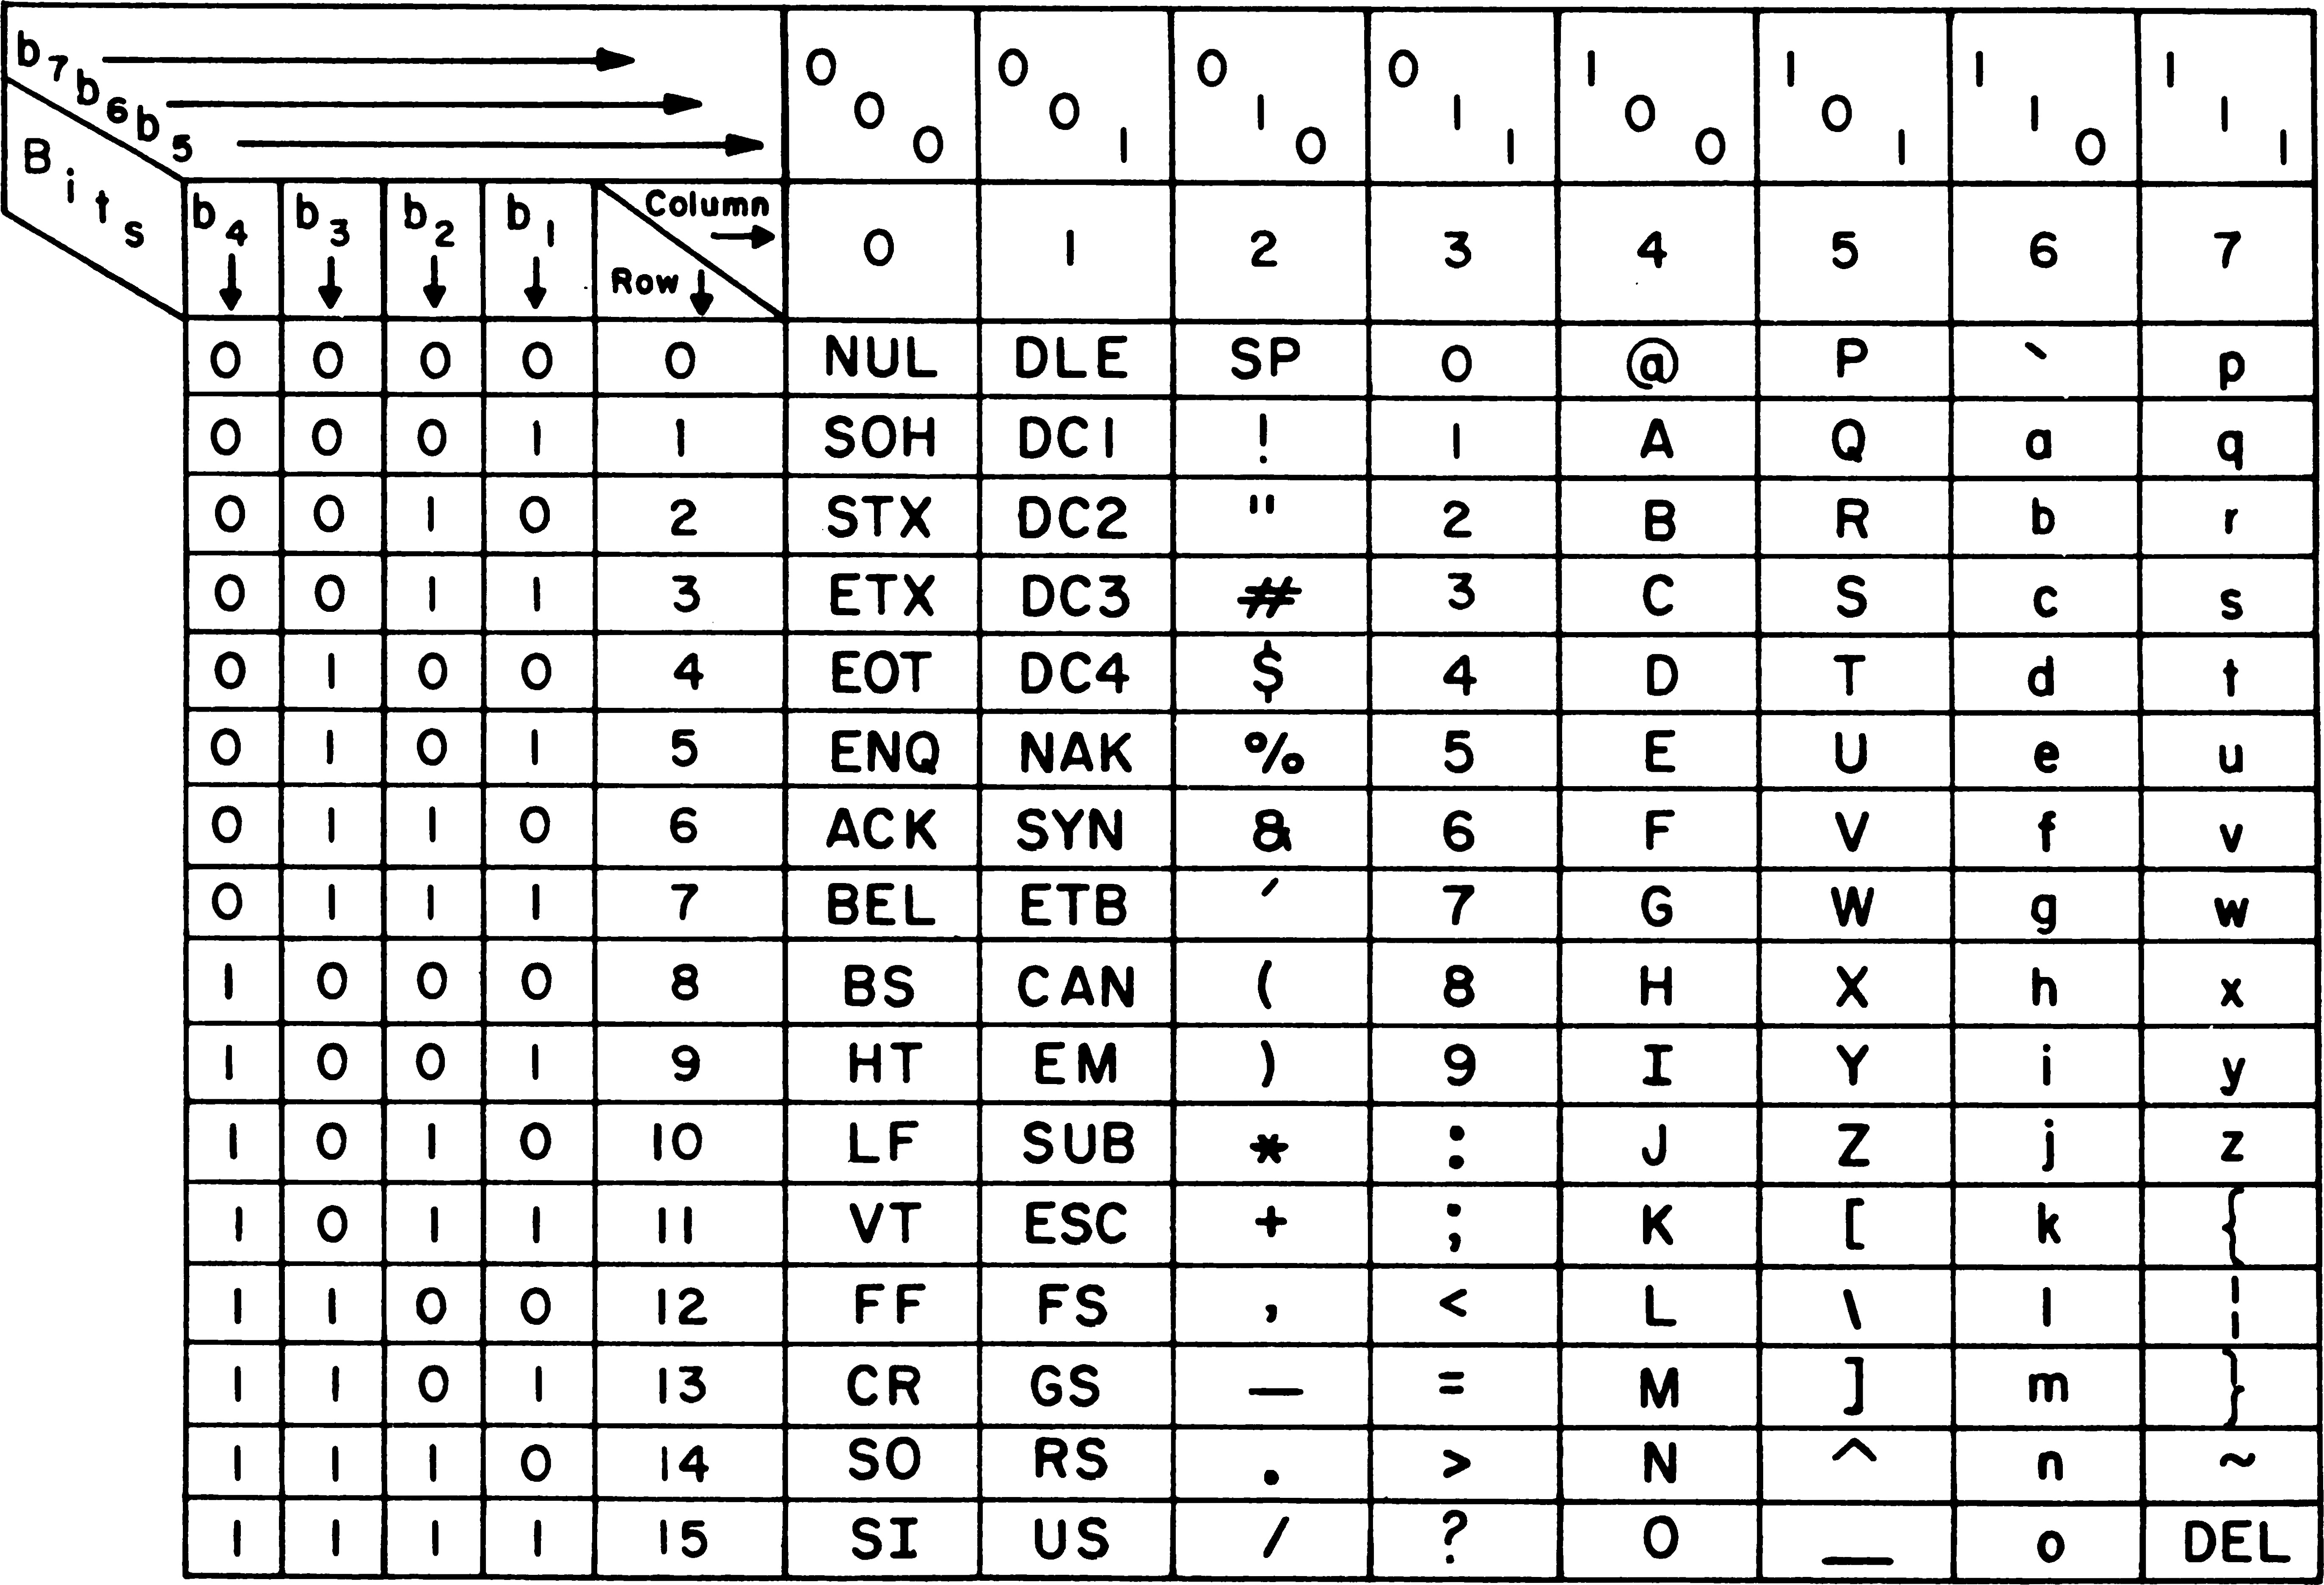
\includegraphics[width=\linewidth]{images/us-ascii.png}
    \caption{ASCII 코드표 ($b_n$은 n번째 bit를 의미) (1967)}
\end{figure}

\subsection{Unicode}

영어를 제외한 언어들을 지원하기 위해,
ASCII코드를 8bit로 확장하거나,
처음부터 새로운 Code Page를 사용하는 등,
각 문화권마다 서로 다른 Code Page를 사용하게 되었다.

같은 문서에 대해 문화권에 따라 문서의 깨짐이 발생하는 등
파편화된 Code Page는 날이 갈수록 심각한 문제를 가지고 왔다.

이에 따라 1991년, Unicode Consortium은 히라가나, 가타카나, 라틴 문자,
한글 등 총 7161자를 포함한 Unicode를 표준화하였다.

이러한 Unicode는 4byte, 즉 32bit에서 정의되는데,
Code Point의 길이를 가변적으로 변화시킴으로서 이 길이를 압축할 수 있다.

압축시키지 않고 4byte그대로 사용하는 Code Page를 UTF-32,
2byte씩 나누어 압축한 Code Page를 UTF-16,
1byte씩 나누어 압축한 Code Page를 UTF-8이라고 한다.
이 중 UTF-8은 ASCII 코드와 호환되어, 세 Code Page중 가장 보편적으로 사용된다.

\begingroup
    \centering
    \begin{longtable}{ || c | c | c | c | c | c || }
        \caption{UTF-8 압축 기법}

        \hline $B_0$ & $B_1$ & $B_2$ & $B_3$ & $B_4$ & $B_5$ \\
        \hline
        \hline 0xxxxxxx & & & & & \\
        \hline 110xxxxx & 10xxxxxx & & & & \\
        \hline 1110xxxx & 10xxxxxx & 10xxxxxx & & & \\
        \hline 11110xxx & 10xxxxxx & 10xxxxxx & 10xxxxxx & & \\
        \hline 111110xx & 10xxxxxx & 10xxxxxx & 10xxxxxx & 10xxxxxx & \\
        \hline 1111110x & 10xxxxxx & 10xxxxxx & 10xxxxxx & 10xxxxxx & 10xxxxxx \\
        \hline
    \end{longtable}
\endgroup

위 도표의 x에 Unicode의 Code Point의 각 bit가 작성되며,
처음에는 1byte를 사용하다가 x의 개수가 부족하면 1byte씩 크기를 늘림으로서 최소한의 byte만을 사용한다.
무엇보다, 1byte만 사용할때, 첫 bit를 0으로 둠으로서 ASCII코드와의 호환성을 가짐을 살펴볼 수 있다.

%\section{글자의 형태, Font}
%\label{sec:fonts}

%\chapter{부록: 아름다운 코드}

%\section{클\-린 코드}
%\label{sec:clean-code}

\end{appendices}

\end{document}